\documentclass[sigconf,10pt,review,anonymous]{acmart}

% AI-SEPS 2019
% https://2019.splashcon.org/home/seps-2019#Call-for-Papers
% 10 pages!

%\usepackage{booktabs} % For formal tables

\usepackage{graphicx}
\usepackage{tabularx}
\usepackage{multirow}
\usepackage{mathtools}
\usepackage{amsmath}
\usepackage{xcolor}
\usepackage{colortbl}
\usepackage{amsmath,amssymb,amsfonts}
\usepackage{algorithm}
\usepackage{numprint}
\usepackage{listings}
\usepackage{tabu}
\usepackage{array}

\let\oldbibitem\bibitem
\def\bibitem{\vfill\oldbibitem}
\usepackage{todonotes}
\usepackage{silence}
\WarningFilter{latex}{Text page}

\newcolumntype{P}[1]{>{\centering\arraybackslash}p{#1}}
\newcolumntype{M}[1]{>{\centering\arraybackslash}m{#1}}

% commented out by Roberto: we should stick to the ACM template
%\usepackage{biblatex}

\graphicspath{ {./figures/} }
 
% Copyright
%\setcopyright{none}
%\setcopyright{acmcopyright}
%\setcopyright{acmlicensed}
%\setcopyright{rightsretained}
%\setcopyright{usgov}
%\setcopyright{usgovmixed}
%\setcopyright{cagov}
%\setcopyright{cagovmixed}

% DOI
%\acmDOI{10.475/123_4}

% ISBN
%\acmISBN{123-4567-24-567/08/06}

%Conference
%\acmConference[WOODSTOCK'97]{ACM Woodstock conference}{July 1997}{El Paso, Texas USA}
%\acmYear{1997}
%\copyrightyear{2016}

%\acmArticle{4}
%\acmPrice{15.00}

% These commands are optional
%\acmBooktitle{Transactions of the ACM Woodstock conference}
%\editor{Jennifer B. Sartor}
%\editor{Theo D'Hondt}
%\editor{Wolfgang De Meuter}

% The default list of authors is too long for headers.
\renewcommand{\shortauthors}{A. Maramzin et al.}

\newcommand{\cpp}{C\texttt{++}}

\newcommand{\totalLoops}{1415}
% This percent is computed in data/reduction.ods
\newcommand{\meanReduction}{45}

\lstdefinestyle{mystyle}{
  backgroundcolor=\color{white},   % choose the background color; you must add \usepackage{color} or \usepackage{xcolor}; should come as last argument
  basicstyle=\ttfamily\footnotesize,        % the size of the fonts that are used for the code
  breakatwhitespace=false,         % sets if automatic breaks should only happen at whitespace
  breaklines=true,                 % sets automatic line breaking
  captionpos=b,                    % sets the caption-position to bottom
  commentstyle=\itshape\color{green},    % comment style
  deletekeywords={...},            % if you want to delete keywords from the given language
  escapeinside={\%*}{*)},          % if you want to add LaTeX within your code
  extendedchars=true,              % lets you use non-ASCII characters; for 8-bits encodings only, does not work with UTF-8
  firstnumber=1000,                % start line enumeration with line 1000
  frame=single,	                   % adds a frame around the code
  keepspaces=true,                 % keeps spaces in text, useful for keeping indentation of code (possibly needs columns=flexible)
  keywordstyle=\color{blue},       % keyword style
  language=C,                 % the language of the code
  morekeywords={*,...},            % if you want to add more keywords to the set
  numbers=none,                    % where to put the line-numbers; possible values are (none, left, right)
  numbersep=5pt,                   % how far the line-numbers are from the code
  numberstyle=\tiny\color{grey}, % the style that is used for the line-numbers
  rulecolor=\color{black},         % if not set, the frame-color may be changed on line-breaks within not-black text (e.g. comments (green here))
  showspaces=false,                % show spaces everywhere adding particular underscores; it overrides 'showstringspaces'
  showstringspaces=false,          % underline spaces within strings only
  showtabs=false,                  % show tabs within strings adding particular underscores
  stepnumber=2,                    % the step between two line-numbers. If it's 1, each line will be numbered
  stringstyle=\color{purple},      % string literal style
  tabsize=2,	                   % sets default tabsize to 2 spaces
  title=\lstname                   % show the filename of files included with \lstinputlisting; also try caption instead of title
}

\lstset{style=mystyle}

%\bibliographystyle{ACM-Reference-Format}
%\addbibresource{main.bib}

\begin{document}

\title{``It Looks Like You're Writing a Parallel Loop''}
\subtitle{A Machine Learning Based Parallelisation Assistant}

\author{Aleksandr Maramzin, Christos Vasiladiotis, Roberto Casta\~neda Lozano, Murray Cole, Bj\"orn Franke}
\affiliation{%
  \institution{The University of Edinburgh}
  \streetaddress{Informatics Forum, 10 Crichton Street}
  \city{Edinburgh}
  \state{Scotland}
  \postcode{EH8 9AB}
}
\email{(s1736883,s1576261)@sms.ed.ac.uk, (roberto.castaneda, mic, bfranke)@ed.ac.uk}

%
% The code below is generated by the tool at http://dl.acm.org/ccs.cfm.
% Please copy and paste the code instead of the example below.
%
%\begin{CCSXML}
%<ccs2012>
% <concept>
%  <concept_id>10010520.10010553.10010562</concept_id>
%  <concept_desc>Computer systems organization~Embedded systems</concept_desc>
%  <concept_significance>500</concept_significance>
% </concept>
% <concept>
%  <concept_id>10010520.10010575.10010755</concept_id>
%  <concept_desc>Computer systems %organization~Redundancy</concept_desc>
%  <concept_significance>300</concept_significance>
% </concept>
% <concept>
%  <concept_id>10010520.10010553.10010554</concept_id>
%  <concept_desc>Computer systems organization~Robotics</concept_desc>
%  <concept_significance>100</concept_significance>
% </concept>
% <concept>
%  <concept_id>10003033.10003083.10003095</concept_id>
%  <concept_desc>Networks~Network reliability</concept_desc>
%  <concept_significance>100</concept_significance>
% </concept>
%</ccs2012>
%\end{CCSXML}

%\ccsdesc[500]{Computer systems organization~Embedded systems}
%\ccsdesc[300]{Computer systems organization~Redundancy}
%\ccsdesc{Computer systems organization~Robotics}
%\ccsdesc[100]{Networks~Network reliability}

\begin{abstract}
% what is the problem
  Despite decades of research into parallelising compiler technology, software parallelisation remains a largely manual task where the key resource is expert time. 
%  
%  Parallelisation involves several crucial stages, including code profiling, analysis, and eventually transformation into a parallel form. 
%  
  In this paper we focus on the time-consuming task of identifying those loops in a program, which are both worthwhile and feasible to parallelise. 
%  
  We present a methodology and tool which make better use of expert time by guiding their effort directly towards those loops, where the largest performance gains can be expected while keeping analysis and transformation effort at a minimum.
  
% what is our solution
  We have developed a novel parallelisation assistant that provides programmers with a ranking of all loops in a program based on their overall merit. This metric combines for each loop its potential contribution to speedup and an estimated probability for its successful parallelisation. This probability is predicted using a machine learning model.

  We have trained trained, validated, and tested our machine learning model on~\numprint{\totalLoops{}} labelled loops and demonstrate a prediction accuracy of greater than~90\%. We have evaluated our parallelisation assistant against sequential C applications from the SNU NAS benchmark suite. We show that our novel methodology achieves results comparable to those from expert programmers while requiring the expert to examine fewer loops, i.e.\ it requires less expert time. On average, our assistant reduces the number of loops to inspect manually by~\meanReduction{}\% before reaching expert-level parallel speedup. 
  
  %It can also  achieves better results (better parallelization) if we allow the same expert time (if true!)

%% \quad Since automatically parallelizing compilers have failed to deliver significant performance improvements, programmers are still forced to parallelize legacy software manually for all but some niche domains. Rather than hoping for an elegant silver bullet, we acknowledge the role of a human expert in the parallelization process and develop a \textit{smart} parallelization assistant.\newline\null
%% \quad In its essence our assistant is yet another application of machine learning techniques to the field of optimizing compilers, which tries to predict the parallelisability property of program loops.
%% We use a version of NAS Parallel Benchmarks (NPB) hand-annotated with OpenMP parallelisation pragmas to train our model. We show that it is possible to achieve a good prediction accuracy of around 90\% for our problem using only static program features. We outperform all available baseline random predictors working at an accuracy ranging between 40\% and 70\%. To get a real practical application of our techniques, we integrate our trained ML model into 2 assistant schemes. Our schemes mitigate the effects of ineradicable statistical errors and make them not that critical. As a result we extend capabilities of Intel \cpp{} compiler in the task of parallelism discovery and increase the amount of parallelism found in SNU NPB benchmarks from 81\% to 96\%. The second scheme is basically an assistant, which directs programmer efforts by pointing the loops, which are the most highly likely to be parallelisible and profitable as well. Thus, decreasing the efforts and time it takes to parallelize a program manually.

%
%Parallelising compilers comprise powerful program analyses, yet they fail to deliver a parallel speedup on real-world programs outside the domain of Fortran-style array based computations due to the limits of static dependence and profitability analyses. Decades of intensive research have not yet delivered a breakthrough, and we do not expect a major breakthrough in static analysis in the near future. In order to accelerate a software a programmer still has to manually analyse and parallelise it. At the same time, the field of machine learning (ML) has made a massive progress and ML techniques are, in fact, already used in parallelising compilers to support profitability analysis and scheduling decisions. In this work we apply ML to predict parallelisability property of program loops and to guide a human effort of software parallelisation.\newline\null
%\quad We use a version of NAS Parallel Benchmarks (NPB) annotated with OpenMP parallelisation pragmas to train our model to predict loop parallelisability property. We show that using only static program features we can achieve the average prediction accuracy of around 90\% against various baselines (random, most frequent, etc.) ranging from 40\% to 70\%. Inherent to all statistical methods false positives comprise around 6\% of cases. To eliminate the danger of false positives we require a final programmer approval and propose 2 schemes of providing a programmer with a parallelisation feedback. The first scheme enhances Intel \cpp{} Compiler (ICC) parallelism discovery in SNU NAS benchmarks from 81\% to 96\% of all SNU NPB parallel loops. The second takes benchmark profiles and provides a programmer with a loop rankings to follow in benchmark parallelisation. Enhanced ranking allows a programmer to converge to the best achievable performance on a benchmark faster, than by following a mere profile based order.
%Here: Novel use of ML in parallelisation to guide human effort: Once all
%automatically parallelisable loops have been parallelised using state-of-the-art
%auto-parallelisers, ML predicts which loops to parallelise next. 
%Evaluated and outlook
%In this work we 
%All modern hardware is highly parallel, but in order to fully utilise availability of all these resources software must be parallel as well. There are numerous approaches to the task of software parallelisation ranging from manual approaches to fully automatic ones. In this work we investigate a relatively new approach to the task of software parallelisation: a machine learning assisted one. We use a version of NAS Parallel Benchmarks annotated with OpenMP parallelisation pragmas to train our model to predict loop parallelisability. We achieve 93\% generalised prediction accuracy with a baseline (random predictor) around 60\%. We study parallelisability of NAS benchmarks and its utilisation with Intel \cpp{} Compiler (ICC) and propose a scheme, which might be used to supplement ICC with a ML-based tool. Proposed scheme increases ICC parallelisation coverage in the NAS Parallel Benchmarks from 86\% to 99\% and comes close to its algorithmic limit. After that we show, that for majority of NAS benchmarks this parallelisation coverage increase transforms into the actual performance improvements as well. We achieve an average speedup of 2.5x relative to the state-of-the-art parallelising Intel \cpp{} compiler and come closer to 3.5x average speedup of the expert hand-parallelised version.

\end{abstract}

%
% Keywords. The author(s) should pick words that accurately describe the work being
% presented. Separate the keywords with commas.
%\keywords{datasets, neural networks, gaze detection, text tagging}

\maketitle

\section{Introduction}

% problem: the need for manual parallelisation, auto-parallelisation does not deliver desired performance improvements

Parallel hardware is ubiquitous through the entire spectrum of computing
systems, from low-end embedded devices to high-end supercomputers.
%
Yet, most of the existing software is written in a sequential fashion.
%
Despite decades of intensive research in automatic software
parallelisation~\cite{6813266}, fully exploiting the potential of modern multi- and many-core hardware still requires a significant manual effort.
%
Given the difficulty of the obstacles faced by automatic parallelisation today,
we do not expect that programmers will be liberated from performing manual
parallelisation in the near future~\cite{Larsen:2012:PML:2410141.2410600}.

% solution: parallelisation assistant

This paper introduces a novel parallelisation assistant that aids the programmer in the process of parallelising a program in the frequent case where automatic approaches fail to do so.
%
The assistant reduces the manual effort in this process by presenting the
programmer a ranking of the program loops that are most likely to 1) require little or no effort for successful parallelisation and 2) improve the program's performance when parallelised.
%
Thus, it improves over the traditional, profile-guided process by also taking into account how \textit{likely} it is that each of the profiled loops can be parallelised.

% how?

At the core of our parallelisation assistant resides a novel machine-learning (ML) model of loop parallelisability.
%
Loops are compelling candidates for parallelisation, as they are naturally
decomposable and tend to capture most of the execution time in a program.
%
Furthermore, focusing on loops allows the model to leverage a large amount of
specific analyses available in modern compilers, such as generalised iterator
recognition~\cite{Manilov:2018:GPI:3178372.3179511} and loop dependence analysis~\cite{Jensen:2017:ILD:3132652.3095754}.
%
The model encodes the result of these analyses together with basic properties of the loops as machine learning \textit{features}.

The loop parallelisability model is trained, validated, and tested
on~\numprint{\totalLoops{}}~loops from the SNU NAS Parallel
Benchmarks~\cite{Seo:2011:PCN:2357490.2358063}.
%
The loops are labelled using a combination of expert OpenMP~\cite{Dagum:1998:OIA:615255.615542}
annotations and optimisation reports from Intel \cpp{} Compiler (ICC), a
production-quality parallelising compiler.
%
The model is evaluated on multiple machine learning algorithms, including tree-based methods, support vector machines, and neural networks.
%
The evaluation shows that -- despite the limited size of the data set -- using
support vector machines allows the model to achieve a prediction accuracy higher than 90\%.
%
% Note: the "detected parallelism increase" is 945/995 - 812/995 = 0.1336683417.
%
The model improves over ICC: Across the sequential C version of the SNU NAS benchmark suite it detects 13\% more parallel loops. Albeit this improvement comes at the cost of introducing \textit{false positives}, where non-parallelisable loops are misclassified as parallelisable. However, the false positive rate is low with 7\%. We feel this is acceptable as our parallelisation assistant does not automatically restructure code, but the final parallelisation is in the hands of the expert users. 
\todo{(FIXME: taken from~Figure~\ref{fig:accuracy_loocv}, double-check these numbers)}

% TODO: mention that we use standard techniques for feature extraction,
% hyper-parameter tuning, and cross-validation?

The parallelisation assistant combines inference on the parallelisability model
with traditional profiling to rank highest those loops with a high likelihood of being parallelisable and impacting the program's performance.
%
An evaluation on seven programs from the SNU NAS benchmark suite shows that
the programs' performance tends to improve faster as loops are parallelised in
the ranking order suggested by our parallelisation assistant compared to a traditional ordering based on profiling.
%
On average, following the order suggested by the assistant reduces
by~\meanReduction{}\% the number of loops that need to be analysed manually to
achieve expert-level speedup.
%
Given the high level of expertise involved in manual analysis, such a reduction
can translate into substantial development cost savings.

%% \quad There is a number of well-known problems in the field of parallel software engineering, which compose the ground our work grows on. Parallel hardware is omnipresent in the whole spectrum of computers from low end devices up to the high end supercomputers. Yet, in order to utilise all these available hardware capabilities the software has to be parallel as well. Unfortunately, the legacy software is written in a sequential fashion and in order to make it run faster we either have to parallelise it manually or rely on automatic parallelisation techniques. Both approaches have their pros and cons. The former require parallel programming expertise on top of the application domain knowledge, the latter is limited to the narrow niche of scientific FORTRAN-like codes. Decades of intensive research have not yet delivered a breakthrough, and we do not expect a major breakthrough in automatic parallelisation in the near future. In order to accelerate a software a programmer still has to manually analyse and parallelise it. Indeed, as our experiments show (see section [?]), even the state-of-the-art Intel \cpp{} compiler cannot achieve significant performance improvements on highly parallel by their nature NAS Parallel Benchmarks (NPB). Meanwhile, the field of machine learning (ML) has made a massive progress and continuously finds itself to be effective and practical in a growing set of application areas. ML based techniques are not new to the field of optimising compilers either. As survey [?] shows ML techniques have been applied to tasks ranging from the selection of the best compiler flags to choosing the most optimal mapping of parallelism onto heterogeneous hardware resources.\newline\null
%% \quad In our work we acknowledge the role of a human programmer in the software parallelisation process and develop a supplementary assistant guiding the human efforts by highlighting program loops, which are highly likely to be parallelisable and profitable as well. Our tool targets the phase of parallelism discovery 


%% For several decades, parallelising compilers have been the subject of intensive academic research \cite{XXX} and industrial investment \cite{XXX}. Yet, for most real-world applications they fail to deliver parallel performance \cite{XXX}.


%% In this paper we take a different approach: We acknowledge the role of the human expert in the parallelisation process, and develop a machine learning based assistant guiding the users to focus their resources on those loops most likely to result in a positive return-of-investment (ROI). We do not aim to completely automate parallelisation including program analysis and transformation, but instead assist the user by suggesting an ordered ranking of loops for manual parallelisation, where this ordering considers both the estimated effort and profit of parallelising each loop in turn.

\subsection{Motivating Example}

Consider the sequential C implementation of the \textit{Conjugate Gradient (CG)} program from the SNU NAS benchmarks.
%
Table~\ref{tab:ranking} shows the top three CG loops as ranked by the Intel
Profiler (based on their execution time) and by our parallelisation
assistant (additionally taking into account predicted parallelisability).
%
Both rankings include the same loops, but, crucially, the loops are \textbf{ranked in a different order}.
%
Among the three loops, only \texttt{cg.c:509} (marked in bold in the table) is
parallelisable, while the other two loops (\texttt{cg.c:326} and
\texttt{cg.c:484}) are not.

\begin{table}
  \caption{Ranking of the top three CG loops.}
  \label{tab:ranking}
  \begin{minipage}{\columnwidth}
  \begin{center}
    \begin{tabu}{cc|ccc}
      \hline
      \rowfont{\bfseries}
      \multicolumn{2}{c|}{profiler} & \multicolumn{3}{c}{assistant} \\\hline
      \rowfont{\bfseries}
      loop & ranking & loop & ranking & parallel \\\hline
      \texttt{cg.c:326} & 0.93 & \textbf{\texttt{cg.c:509}} & \textbf{0.34} & 85\%\\
      \texttt{cg.c:484} & 0.91 & \texttt{cg.c:326} & 0.17 & 29\%\\
      \textbf{\texttt{cg.c:509}} & \textbf{0.89} & \texttt{cg.c:484} & 0.05 & 8\%\\
    \end{tabu}
  \end{center}
  \end{minipage}
\end{table}%

Following the profiler ranking as in traditional profile-guided parallelisation
(two first columns in Table~\ref{tab:ranking}), the loops \texttt{cg.c:326} and
\texttt{cg.c:484} are selected first for manual analysis.
%
The analysis determines that these loops are not parallelisable, due to
inter-iteration dependencies and side effects caused by system calls (see
Listing~\ref{lst:main_iter}).
%
Finally, manual analysis of loop \texttt{cg.c:509} (see
Listing~\ref{lst:reduction}) recognises that it computes an array of reductions
and is thus parallelisable.
%
Just parallelising this loop speeds up CG by a factor of 2.8, which is 80\% of
the speedup obtained by an expert parallelisation of the entire program.

In contrast, our parallelisation assistant (two last columns in
Table~\ref{tab:ranking}) predicts that loop \texttt{cg.c:509} is parallelisable
(with a likelihood of 85\%) while loops \texttt{cg.c:326} and \texttt{cg.c:484} are not (likelihood of just 29\% and 8\%).
%
Consequently, it ranks the loop \texttt{cg.c:509} at the top, allowing the user to achieve the same program speedup without having to analyse loops \texttt{cg.c:326} and \texttt{cg.c:484}.
%
% Note: the 100 lines of code are counted using 'cloc code/cg-326.c'.
%
The manual effort savings are significant, considering that \texttt{cg.c:326} is an outermost loop consisting of 100+ lines of code (including its callee function
\texttt{conj\_grad} where \texttt{cg.c:484} and \texttt{cg.c:509} are defined)
whereas \texttt{cg.c:509} is a relative small loop consisting of just the six lines shown in Listing~\ref{lst:reduction}.

\begin{figure}[t]
\begin{lstlisting}[caption={\texttt{cg.c:326}. Longest running loop in CG. The loop cannot be parallelised due to
inter-iteration dependences and side effects caused by system calls.},label={lst:main_iter},language=C]
for (it = 1; it <= NITER; it++) {
  ...
  if (timeron) timer_start(T_conj_grad);
  conj_grad(colidx,rowstr,x,z,a,p,q,r,&rnorm);
  if (timeron) timer_stop(T_conj_grad);
  ...
  printf("    %5d       %20.14E%20.13f\n", it, rnorm, zeta);
  ...
}
\end{lstlisting}

\begin{lstlisting}[caption={\texttt{cg.c:509}. Longest running loop in CG \emph{that can be parallelised}.},label={lst:reduction},language=C]
for (j = 0; j < lastrow-firstrow+1; j++) {
  suml = 0.0;
  for (k = rowstr[j]; k < rowstr[j+1]; k++)
    suml = suml + a[k]*p[colidx[k]];
  q[j] = suml;
}
\end{lstlisting}
\end{figure}



\subsection{Contributions}

In this paper we are making the following contributions:
%
\begin{itemize}
\renewcommand\labelitemi{$\vartriangleright$}
\renewcommand\labelitemii{$\bullet$}
\item We develop and train a machine learning model, which can be used to predict the probability with which sequential C loops can be parallelised,
\item we integrate profiling for hotspots with our novel ML model into a parallelisation assistant, which guides the user through a ranked list of loops for parallelisation, and
\item we demonstrate that our tool and methodology increases programmer productivity by identifying parallel loop candidates better than existing state-of-the-art approaches.

%Designed an ML based model of loop parallelisability quantifying the latter %(Section~\ref{predicting_parallel_loops}) and ranking program loops
%    \begin{itemize}
%    \item Devised loop parallelisability metrics (ML loop features)
%    \item Prepared a labelled training set with classification labels
%    derived from SNU NPB OpenMP \textit{\#pragmas} as well as Intel Compiler %optimisation reports
%    \item Set and tuned an ML train/test methodology
%    \end{itemize}
%\item Conducted a thorough evaluation of the model demonstrating prediction %accuracy
%  higher than 90\% on~\numprint{\totalLoops{}}~loops from the SNU NAS Parallel
%  Benchmarks (\textcolor{red}{Section~4})
%\item Integrated the model into a parallelisation assistant scheme that %automatically ranks promising loops by combining profiling information and %model inference (\textcolor{red}{Section~5})
%    \begin{itemize}
%    \item Demonstrated improved parallelism discovery capabilities of %assistant in comparison with Intel Compiler 
%    \end{itemize}
%\item Deployment of the assistant on SNU NAS Parallel Benchmarks demonstrating %its potential to ease parallelisation process and converge to the maximum %attainable performance faster
%    \begin{itemize}
%    \item Conducted a performance study of SNU NPB with the state-of-the-art %Intel Compiler
%    \item Parallelisied SNU NPB following profiler and assistant suggested %loop orders and plotted performance convergense curves
%    \end{itemize}
%
% a demonstration of the assistant's potential to reduce the manual effort
%  involved in the traditional profile-guided parallelisation methodology
%  (\textcolor{red}{Section~6}).
\end{itemize}
%% 1) We show that it is possible to learn loop
%% have successfully learnt the parallelisability property o
%% 2) We conduct a study of Intel Compiler's behaviour on SNU NPB benchmarks. We summarise the exact optimizations applied (see section [?]), classify missed parallelisation opportunities (see section [?]) and
%% \subsection{Overview}

%% \subsection{Paper structure}
%% \quad The most substantial part of this work was aimed at the creation of machine learning (ML) based model, capable of accurate prediction of loop parallelisability property. Section \ref{predicting_parallel_loops} describes all the details of machine learning part including the features we chose and the exact training/testing methodology we used. But even close to perfect prediction accuracy is not enough, if we cannot find a real practical application to utilise our predictor. Section \ref{practical_applications} proposes 2 complementary schemes we might integrate our predictor into. The first scheme helps Intel ICC compiler to discover additional parallelism. The second scheme is basically software manual parallelisation assistant working with a program profile and directing human efforts at the most likely to be parallelisible (and profitable as well) loops. Section \ref{evaluation} presents a quantitative report on our work.  


%\section{Background}

%\subsection{Parallelism Discovery}

%\subsection{Profitability Analysis}

%For example, SUIF \cite{Wilson:1994:SIR:193209.193217} uses a simple heuristic based on the product of statements per loop iteration and number of loop iterations to decide whether a parallelizable loop should be scheduled to be executed in parallel. In contrast, \cite{Tournavitis:2009:THA:1542476.1542496} uses a machine learning based heuristic, which consumes \textit{dynamic} program features collected in a separate profiling stage, to decide if and how a potentially parallel loop should be scheduled across multiple processors.

\section{Predicting Parallel Loops}
\label{predicting_parallel_loops}

%\quad This section describes the exact way we applied supervised machine learning (ML) techniques to the problem of loop parallelisability classification. Here we describe the features we choose to represent program loops and the way we collect our data, as well as the whole ML train/test \textit{methodology}. The methodology consists of a number of stages arranged in a \textit{pipeline} (data extraction, data preprocessing, automatic feature selection, ML model selection and the search of its hyper-parameter spaces, training/validation/testing, etc.). All technical background on ML can be found in the book \cite{James:2014:ISL:2517747}.\newline\null
%\quad In order to achieve the best ML performance our features and the exact parameters of methodology have been iteratively tuned and refined with the help of K-fold CV. Predictive \textit{accuracy}, \textit{recall} and \textit{precision} scores were used as selection criteria. To get the most accurate and honest assessment of our ML models we kept the testing data hidden and used only the training data during all ML pipeline stages. Following subsections present the final results rather than the path towards them.


% \subsection{Overview}
% \label{ml_overview}
\todo{Shrink this entire section!}

We approach the prediction of parallel loops as an \textbf{supervised machine learning classification problem}: Based on sequential reference applications and their manually parallelised counterparts as well as Intel's parallelising C/C++ compiler we create a training set of parallelisable and non-parallelisable loops and their features. We use this training data to train a machine learning model, which links feature vectors describing the loops and their observed parallelisability. We then use the trained model as a predictor: for each new loop we determine its feature vector and then predict whether or not the loop is parallelisable using the previously trained model.



%\textit{create an ML based model of loop parallelisability and train it to classify loops of Seoul National University implementation \cite{snu-npb-benchmarks} of NAS Parallel Benchmarks \cite{nasa-parallel-benchmarks} as parallelizable or not.}\newline\null 
%\quad We used facilities of \textit{scikit-learn} \cite{scikit-learn} Python library for all ML related tasks. To conduct various ML training/testing experiments in the search of the best ML model we developed a scripting framework taking an input data (train and test) along with an ML pipeline INI configuration file. Configuration file allows us for a flexible change in the settings of an experiment (ML model to use, its hyper-parameter search space, the exact automatic feature selection methods, etc.). The following sections give a detailed description of all ML pipeline stages.

\subsection{Loop Analysis \& Feature Extraction}
\label{loop_analysis_and_features}

%\begin{comment}
%\quad We base our feature engineering efforts on the vast body of work done in the field of optimising compilers. Particularly in the domain of program dependence analysis \cite{Kennedy:2001:OCM:502981}. 
%We dump PDGs in a dot format and systematically use these visualisations in our work in order to debug and decide on the best features to use.
%\end{comment}

For the purpose of machine learning, program loops are represented by numerical \textit{feature vectors}. We derive these features using standard compiler analyses operating on the Program Dependence Graph (PDG) \cite{Ferrante:1987:PDG:24039.24041} of a loop. These features aim to capture loop information obtained using general program dependence analysis theory \cite{Kennedy:2001:OCM:502981}. Figure \ref{fig:pdg} shows an example of a PDG built for a simple loop and visualised with our tool.

\begin{figure}[ht]
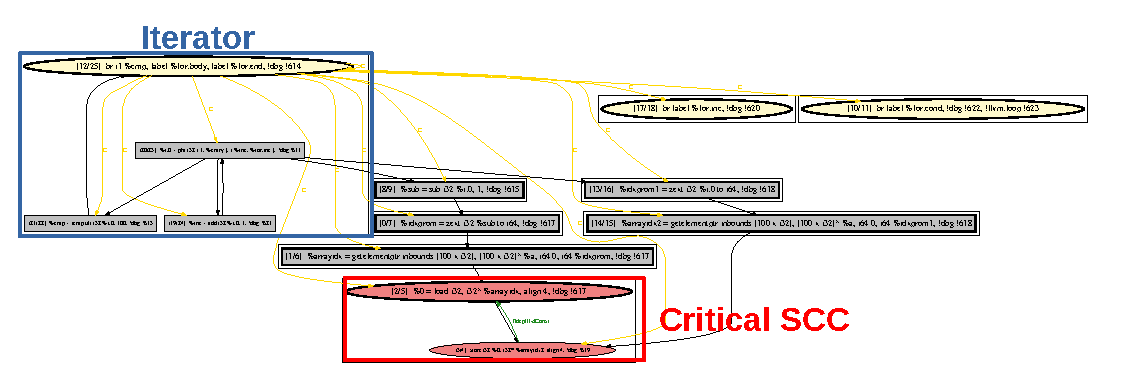
\includegraphics[width=0.45\textwidth]{figures/pdg_example.pdf}
\caption{Example of PDG of a simple loop with a cross-iteration dependency built and visualised by our tool.}
\label{fig:pdg}
\end{figure}

%\quad One of the most important parts in applying ML techniques to a given problem is the \textit{feature engineering} task. In our project we need to pick the right program loop features, which are the most reflective of loop parallelisability property. In the task of coming up with a set of loop features we are guided by general program dependence analysis theory \cite{Kennedy:2001:OCM:502981}, the exact types of loops present in SNU NPB benchmarks and Intel \cpp{} compiler optimisation reports.\newline\null
%\quad There is a range of SNU NPB loops, which escape Intel compiler parallelisation for different reasons: indirect array references, unrecognised reductions on arrays, pointers with statically unknown memory locations, etc. But all that range of reasons is going to ultimately materialise into data and control dependencies present between loop instructions, represented as edges on the Program Dependence Graph (PDG) \cite{Ferrante:1987:PDG:24039.24041} of a loop. Figure \ref{fig:pdg} shows an example of a PDG built for a simple loop and visualised with our tool.\newline\null

We construct the PDG on a program's LLVM IR and apply standard dependence analysis. In addition we use \textit{generalised loop iterator recognition} \cite{Manilov:2018:GPI:3178372.3179511} to separate out \textit{loop iterators} from \textit{loop payloads}. This enables us to define and extract features relating to each of those loop components. In total, we extract a set of 74 static loop features which are based on structural properties of PDG and the types of instructions constituting them. Table \ref{tab:loop_features} provides a summary of these features.

%\quad The PDG graph consists of LLVM IR instructions as nodes and different sorts of dependencies between them as graph edges. Dependence relation lies at the the very essence of loop parallelisation, on the other hand just counting the number of dependence edges in the PDG of a loop is not enough to make decisions about loop parallelisability. Dependence relations might exist only withing one loop iteration or span across multiple, thus preventing parallelisation.\newline\null
%\quad To refine our features we use the work on \textit{generalised loop iterator recognition} \cite{Manilov:2018:GPI:3178372.3179511}. Generalised iterator recognition analysis separates \textit{loop iterator} from the actual \textit{loop payload} providing us with finer loop partitions to base our features on. As work \cite{Manilov:2018:GPI:3178372.3179511} explains, loop iterator is a \textit{strongly connected component (SCC)} on the PDG with no incoming dependence edges. There are SCCs in the payload as well. Usually they consist of just 1 instruction, but when we have a cross-iteration dependency they tend to grow larger and form a cycle. We call such SCCs \textit{critical}, as ones preventing parallelisation. Figure \ref{fig:pdg} highlights both the iterator and the critical SCC present in the example loop. Inner loop iterators tend to appear as critical SCCs for the outer loop as well. To separate these cases we use \textit{inner loops number} and \textit{loop depth} as separate ML features.\newline\null  
%\quad The feature engineering process has been conducted iteratively and has been guided by the change in ML models predictive performance with the addition of one feature or the other. This process involved several methods. First, we tried to capture in our features the differences between PDG visualisations for parallel and non-parallel loops. Then we studied the source code of SNU NPB benchmarks along with ICC optimization reports and tried to understand why ICC failed to parallelize some of SNU NPB loops and transfer those insights into reflective features.\newline\null
%\quad We ended up with a set of 74 static loop features, which are based on the structural properties of PDG and the types of instructions constituting them. Table \ref{tab:loop_features} summarizes the main groups of devised features.\newline\null
\quad Many of our features have a simple and intuitive motivations behind them. Loop proportion related features are backed up by the the fact, that bigger loops are harder to parallelize. Big iterators contain complex cross-iteration transitions (e.g linked-list update), unknown iteration numbers, etc. Critical SCCs limit loop parallelization further. Cohesion features do not have an apparent intuition. They characterise how tightly components of loops are coupled together in terms of the number of edges between them. Loop dependencies number features count the number of edges in different loop parts as well as their types. Loop instructions nature characterise the types of loop instructions, assigning more importance to memory reads/writes, calls, branches. Uninlined funtion calls usually prevent loop parallelization. Intensive memory work (memory read/write fraction features) complicates parallelization as well.   

\begin{table*}[!ht]
  \begin{minipage}{\linewidth}
  \begin{center}
    \begin{tabu}{M{3cm}M{5cm}M{8cm}}
      \hline
      \rowfont{\bfseries}
      Feature groups & Features & Description\\\hline
      \multirow{3}{*}{Loop Proportions} & Absolute Size & the number of LLVM IR instructions\\%\hline
      & Payload Fraction & $\frac{payload instructions number}{whole loop instructions number}$\\%\hline
      & Proper SCCs Number & number of payload SCCs with more than 1 instruction\\\hline
      Loop Dependencies & \multicolumn{2}{M{13cm}}{The number of PDG edges corresponding to different dependence classes: read/write order (\textbf{True}, \textbf{Anti}, \textbf{Output}), dependency media (\textbf{Register}, \textbf{Memory}, \textbf{Control}), other (\textbf{Confused}, \textbf{Cross-Iteration})}\\\hline
      \multirow{2}{*}{Loop Cohesion} & Iterator/Payload & $\frac{Num of Edges Between Iterator/Payload}{Total Loop Edges Num}$\\
        & Critical/Regular Payload & $\frac{Num of Edges Between Critical/Regular Payload}{Total Loop Payload Edges Num}$\\
        \hline
      \end{tabu}
  \end{center}
  \end{minipage}
  \caption{Static features used for the characterisation of loops.}
  \label{tab:loop_features}
\end{table*}%


%\subsection{Feature Extraction}
%\label{feature_extraction}
%\quad To extract all devised loop features from SNU NPB benchmarks and get the train/test data set we developed \textbf{PParMetrics (Pervasive Parallelism Metrics)} tool, based on the LLVM compiler infrastructure \cite{llvm-compiler-infrastructure}\cite{Lattner:2004:LCF:977395.977673}. The tool is a set of LLVM function passes working on the SSA-based LLVM IR and can be found on the GitHub \cite{github-ppar-tool}. The tool works by building data, memory and control dependence graphs (DDG, MDG, CDG) and combining them into the final program dependence graph (PDG) \cite{Ferrante:1987:PDG:24039.24041} for all loops found in program functions. Once all graphs are built we run the search of strongly-connected components (SCCs) on them and recognise loop iterators. The final step is to traverse all these graphs computing devised metrics (ML features) and dump all that information into the file to be later fed into scikit-learn based ML scripts.


\subsection{Feature Selection}
\label{feature_selection}
%\quad The feature engineering task resulted into a quantitative description of program loops being characterised by feature vectors of length 74. 

To avoid ML model over-fitting we discard irrelevant or redundant features. For this we eliminate features with a low variance score, then we fit a decision tree based model and select features with importance score above a given threshold. We repeatedly run \textit{Recursive Feature Elimination, Cross-Validated (RFECV)} feature selection. This yields the 10 highest ranked features shown in Table \ref{tab:best_features}.

%Our ML pipeline scripts can be configured to apply an arbitrary sequence of different scikit-learn feature selection methods. First we filter out all features with a low variance score, then we fit a decision tree based model and select all features with importance score above the threshold. Then we repeatedly run recursive feature elimination by the cross-validation (RFECV) in an attempt to improve several targets: recall, precision and accuracy scores. Table \ref{tab:best_features} illustrates the relative ranking of the 10 highest scoring features in our automatic feature selection runs. SNU NPB benchmarks contain a lot of uninlined function calls and it is unsurprising that the amount of call instructions in the payload of a loop ranks the highest. Despite the absence of straightforward intuition behind cohesion metrics, they tend to correlate with parallelisation labels well. Loops heavy on memory writes also significantly affect the parallelisability property.

\begin{table}[ht]
  \begin{minipage}{\columnwidth}
  \begin{center}
    \begin{tabu}{ll}
      \hline
      \rowfont{\bfseries}
      \multicolumn{1}{l}{Feature} & \multicolumn{1}{l}{Importance}\\\hline
      payload call fraction & 23.5\\
      iter/payload non-cf cohesion & 18.5\\
      payload mem write fraction & 6.1\\
      loop absolute size & 5.7\\
      critical payload getelemptr count & 5.3\\
      payload mem dep num & 4.0\\
      critical payload non-cf cohesion & 2.9\\
      payload getelemptr fraction & 2.7\\
      critical payload total cohesion & 2.6\\\hline
      \end{tabu}
  \end{center}
  \end{minipage}
  \caption{Relative importance of static loop features, ranked by fitting a tree based ML model.} 
  \label{tab:best_features}
\end{table}%


\subsection{Model \& Hyper-Parameter Selection}
\label{model_selection}

We evaluate several machine learning algorithms in our parallelisation assistant, including tree-based methods like (decision trees (DT), random forests (RFC), boosted decision trees (AdaBoost)), support vector machines (SVC) and neural network based multi-layer perceptron (MLP). In section \ref{evaluation_kfold} we show that these models perform similarly well with SVC and MLP performing slightly better.

%\quad We use several machine learning algorithms available in the scikit-learn library to compare and find the best one. Among these are tree-based methods like (decision trees (DT), random forests (RFC), boosted decision trees (AdaBoost)), support vector machines (SVC) and neural network based multi-layer perceptron (MLP). Section \ref{evaluation_kfold} shows, that all these models perform comparably good with SVC and MLP being slightly better.
%\subsection{Model Hyper-Parameter Selection}
%\label{model_hyper_parameter_selection}

%\quad For any chosen parametric machine learning model we need to pick the right set of model hyper-parameters. 
For each ML model we use exhaustive hyper-parameter grid search and pick the node with the best cross validation score on the training set. We vary grid spaces in an attempt to find the best scoring one. The SVC model tends to vary parameters \textit{C} and $\gamma$, but it almost always chooses an RBF kernel. A multi-layer perceptron works the best with the \textit{relu} activation function, \textit{lbfgs} solver and varying $\alpha$ and network configuration. Tree based methods tend to keep to relatively small depths (5-15). 

\begin{comment}
\begin{table}[h!]
    \centering
    \begin{tabular}[c]{|p{2.0cm}|p{5.0cm}|}
        \hline
        model & hyper-parameter space\\
        \hline
        SVC & \textbf{kernel}: rbf,sigmoid,poly, \textbf{C}: 1,10,$10^2$,$10^3$ \textbf{$\gamma$}: 1,$10^{-1}$,$10^{-2}$,$10^{-3}$,$10^{-4}$\\
        \hline
        DT RFC AdaBoost & \textbf{n\_estimators}: 1,2,5,10,50,100 \textbf{max\_depth}: 1,3,5,7,10,15,20,30,50 \textbf{min\_samples\_split}: 0.05,0.1,0.2,0.5,0.7,0.9 \textbf{min\_samples\_leaf}: 1,5,10,15,30,50,60,70,100 \textbf{max\_features}: 1,5,10,15,30,50,70\\
        \hline
        MLP & \textbf{activation}: logistic,relu,tanh \textbf{solver}: lbfgs,sgd,adam \textbf{hidden\_layes\_sizes}: (5;5),(10),(10;10),(10;5),(5;2),(2;5) \textbf{$\alpha$}: $10^2$,10,1,$10^{-1}$,$10^{-2}$\\
        \hline
    \end{tabular}
    \caption{Hyper-parameter spaces to search for an optimal point for different ML models.}
    \label{tab:hyper_param_space}
\end{table}

\begin{table}
  \begin{minipage}{\columnwidth}
  \begin{center}
    \begin{tabu}{ccc}
      \hline
      \rowfont{\bfseries}
      \multicolumn{1}{c}{Model} & \multicolumn{2}{c}{Hyper-Parameter Space}\\\hline
      \multirow{3}{*}{\textbf{SVC}} & \textit{kernel:} & rbf, sigmoid, poly\\%\hline
      & \textit{C:} & 1, 10, $10^2$, $10^3$\\
      & \textit{$\gamma$:} & 1, $10^{-1}$, $10^{-2}$, $10^{-3}$, $10^{-4}$\\\hline
      \multirow{5}{*}{\textbf{\shortstack[c]{DT\\AdaBoost\\RFC}}} & \textit{n\_estimators:} & 1, 2, 5, 10, 50, 100\\%\hline
      & \textit{max\_depth:} & 1, 3, 5, 7, 10, 15, 20, 50\\
      & \textit{min\_samples\_split:} & 0.05, 0.1, 0.2, 0.5, 0.7, 0.9\\
      & \textit{min\_samples\_leaf:} & 1, 5, 10, 15, 30, 50, 70, 100\\ 
      & \textit{max\_features:} & 1, 5, 10, 15, 30, 50, 70\\\hline
    \end{tabu}
  \end{center}
  \end{minipage}
  \caption{Hyper-parameter spaces to search for an optimal point for different ML models.} 
  \label{tab:hyper_param_space}
\end{table}%

\begin{table}
  \begin{minipage}{\columnwidth}
  \begin{center}
    \begin{tabu}{ccc}
      \hline
      \rowfont{\bfseries}
      \multicolumn{1}{c}{Model} & \multicolumn{2}{c}{Hyper-Parameter Space}\\\hline
      \multirow{3}{*}{\textbf{SVC}} & \textit{kernel:} & rbf, sigmoid, poly\\%\hline
      & \textit{C:} & 1 ... $10^3$\\
      & \textit{$\gamma$:} & 1 ... $10^{-4}$\\\hline
      \multirow{5}{*}{\textbf{\shortstack[c]{DT\\AdaBoost\\RFC}}} & \textit{n\_estimators:} & 1 ... 100\\%\hline
      & \textit{max\_depth:} & 1 ... 50\\
      & \textit{min\_samples\_split:} & 0.05 ... 0.9\\
      & \textit{min\_samples\_leaf:} & 1 ... 100\\ 
      & \textit{max\_features:} & 1 ... 70\\\hline
    \end{tabu}
  \end{center}
  \end{minipage}
  \caption{Hyper-parameter search spaces for various ML models. Only diapason is shown for ease of visualisation.} 
  \label{tab:hyper_param_space}
\end{table}%
\end{comment}

   

\begin{comment}
Model hyper-parameter tuning process consists of several parts. First, we determine the most important hyper-parameters for each ML model being used. Then, we build a grid with these hyper-parameter ranges. To assess each combination of hyper-parameter values, represented as a point on the grid we perform a standard process. We split our entire set of SNU NAS loops into training and testing subsets. We then take the training subset and further partition it into K different folds. For each fold we train the model with a set hyper-parameters on the remaining K-1 folds and test it on the chosen fold. We average calculated prediction accuracy scores and pick the best one for each hyper-parameter grid point. Then we take the combination of hyper-parameters, which corresponds to the best score.\newline\null
\quad Once the best performing set of hyper-parameters is chosen using CV on the training set, we train ML model with these hyper-parameters on the whole training set and subsequently test it on the testing set chosen at the very beginning.
\end{comment}

\subsection{Training Data \& ML Model Training}
\label{loop_classification_labels}

% \quad In order to train and test our ML model in a supervised way, we need to provide it with the "right answers" regarding loop parallelisability. The task of getting classification labels for loops of SNU NPB benchmarks is complicated by several factors.\newline\null

For training our ML model we use a total of 1415 loops from the SNU NPB benchmark suite. Out of those loops, 210 have been annotated by (external) human experts with parallel OpenMP \textit{\#pragmas}. We use these annotations as labelled data to indicate ''parallelisable" loops. However, the data is not complete. Human programmers capture only coarse-grain parallelism in the benchmarks, and do not annotate parallelisable, but unprofitable loops. Hence, we complement the training data with the help of Intel's parallelising compiler, which when configured to aggressively detect parallelism, finds additional ''parallelisable" loops. We combine the results into our training set comprising a total 1415 loops, of which 995 are labelled as ''parallelisable".  We then use K-fold and Leave-One-Out Cross-Validation (LOOCV) to train and test our ML models. 


%and leave a lot of parallelisable loops (parallelisation of which deems unprofitable) unannotated. By using only these 210 "yes" labels, we are risking to mislead our ML model, since it uses only static program features reflecting dependence-based algorithmic parallelisability of program loops, which do not reflect the profitability of their parallelisation. Moreover, the data set is rather unbalanced (210 "yes" vs 1205 "no"). The latter sets the baseline predictive performance we are going to compete with to a very high level of 85\%. The work \cite{fried_ea:2013:icmla} suffers from this. And seems to incline to classify bigger loops as parallelisable. Given the parallel nature of big loops in SNU NPB, that results into high prediction accuracy, which might not hold for a different set of benchmarks.\newline\null
%\quad Due to above considerations we blend an additional knowledge into our parallelisability labels. We use optimisation reports of the Intel compiler as a second source of information. To extract loop parallelisability labels from the Intel compiler's optimisation reports we developed an optimisation report parser \cite{github-icc-parser}. The task presented us with a number of technical challenges. Before ICC can actually parallelise or vectorise a loop, it applies a number of enabling loop transformations such as loop interchange, distribution, tiling, etc. The detailed description of all these transformations can be found in the paper \cite{Bacon:1994:CTH:197405.197406}. Applied to a loop nest, these optimisations might significantly restructure and distribute the parts of a loop across the whole ICC optimisation report. Moreover, ICC might parallelise only certain parts of transformed loop. At the end we considered a loop to be parallelisible by the ICC compiler if the latter hasn't found any dependencies and either vectorised or parallelised it. In the case of distributed loops, all parts must be parallelisible for an original loop to be considered as such. For a final correctness we conducted a manual verification on top of automatically extracted results.\newline\null
%\quad Table \ref{tab:icc_stats} presents a parsing report, which summarises the number of times ICC applied a certain optimisation. The major cells are \textit{parallel} and \textit{icc}, which report the total number of truly parallelisible loops and the number of loops parallelised by ICC. As it can be seen ICC dompiler does not exploit all the parallelism available in SNU NPB benchmarks. Section \ref{evaluation_icc_competition} presents a study of reasons ICC fails to parallelise certain loops.
%\begin{comment}
%\begin{table}[h!]
%    \centering
%    \begin{tabular}[c]{|p{1.7cm}|p{1.7cm}|p{1.7cm}|p{1.7cm}|}
%        \hline
%        total loops & 1415 & parallelised & 653\\
%        \hline
%        parallel & 995 & vectorized & 737\\
%        \hline
%        icc & 812 & parallel deps & 535\\
%        \hline
%        openmp & 210 & vector deps & 266\\
%        \hline
%        distrs & 34 & fusions & 214\\
%        \hline
%        collapses & 58 & tilings & 27\\
%        \hline
%    \end{tabular}
%    \caption{SNU NPB ICC and OpenMP parallelisation statistics. The true %parallel labels are denoted by \textit{parallel}. Number of loops parallelised %by ICC is \textit{icc}. Remaining cells report on different kinds of %optimizations done and reported by the ICC.}
%    \label{tab:icc_stats}
%\end{table}
%\end{comment}
%\begin{table}
%  \begin{minipage}{\columnwidth}
%  \begin{center}
%    \begin{tabu}{cccccc}
%      \hline
%      \rowfont{\bfseries}
%      \multicolumn{2}{c}{\multirow{2}{*}{Labels}} & \multicolumn{4}{c}{Intel %Compiler (ICC)} \\%\hline
%      \rowfont{\bfseries}
%      & & \multicolumn{2}{c}{Optimisation} & %\multicolumn{2}{c}{Parallelisation}\\\hline
%      %loop & ranking & loop & ranking & parallel \\\hline
%      \textbf{total loops} & \textbf{1415} & distrs & 34 & parallel & 653\\
%      \textbf{parallel} & \textbf{995} & fusions & 214 & vector & 737\\
%      \textbf{icc} & \textbf{812} & collapses & 58 & parallel deps & 535\\
%      \textbf{openmp} & \textbf{210} & tilings & 27 & vector deps & %266\\\hline
%    \end{tabu}
%  \end{center}
%  \end{minipage}
%  \caption{Loop classification labels report.}
%  %\caption{Report on loop classification labels derived out of expertly added %OpenMP annotations of SNU NPB benchmarks and ICC optimisation reports. Out of %995 parallelisable loops ICC discovered and parallelised 812.}
%  \label{tab:icc_stats}
%\end{table}%


% \subsection{ML Model Training}
% \label{train_test_methodologies}



%Both have their specific goals and properties.\newline\null
%\quad K-fold CV method blends all the loops from all SNU NPB benchmarks together in the single set and divides it into K equally sized splits. After that the method uses all the possible combinations of K-1 splits to train a model and test it against the one remaining split. Resultant accuracies are averaged to produce the final score. The advantage of that method is that it uses loops from all SNU NPB benchmarks for training and testing. In other words, SNU NPB benchmarks differ in their nature and we use all the available cases and properties to train a model and do not miss any of the information. That leads us to a better overall score. We use that method to tune our model and report its general performance for the same reason as well.\newline\null
%\quad But if we want to utilise our ML models in different practical scenarios (see section \ref{practical_applications}) we have to use separate SNU NPB benchmarks as the whole during model testing. To accomplish that we employ a modified LOOCV method to estimate the predictive performance our models can achieve against separate benchmarks in the set. Here we take all loops in every single benchmark as a testing set and train the model on all loops of 9 remaining benchmarks. The disadvantage of that method is that we exclude the whole benchmark out of the training process. If benchmark has a different nature from the ones we used to train the model, then that comes at the price of reduced accuracy.

\section{ML Predictive Performance}

We evaluate the predictive performance of our trained ML model using K-fold cross validation as discussed in the previous section.

%\quad This section reports on the predictive performance of ML based loop parallelisability model described in the previous section. As has already been described, before we conduct our performance assessment experiments, we have tuned all the parameters of our train/test methodology with the help of K-fold CV and show only the final results.    
%\begin{comment}
%We have 10 SNU NAS benchmarks. We choose one of them and run the oracle training pipeline on the 9 remaining ones. Once the oracle is trained we test it using the chosen unseen benchmark and get parallelisability feedback. Table reports on the performance of out LOOCV method. 
%\end{comment}

\subsection{Cross-Validation}
\label{evaluation_kfold}

In Figure \ref{fig:accuracy_loocv} we show the cross-validation performance of the different ML models on the SNU NPB data set as the whole. Training and testing have been done for different values of K and as shown in Figure \ref{fig:accuracy_kfold} the results are stable across the entire range of K. Similarly, recall and precision scores are equally stable across the range of K. Detailed figures are shown in Table \ref{tab:average_accuracy}. This provides us with confidence that our approach has yielded a robust ML model capturing the characteristics of loop parallelisation.

\begin{figure}[ht]
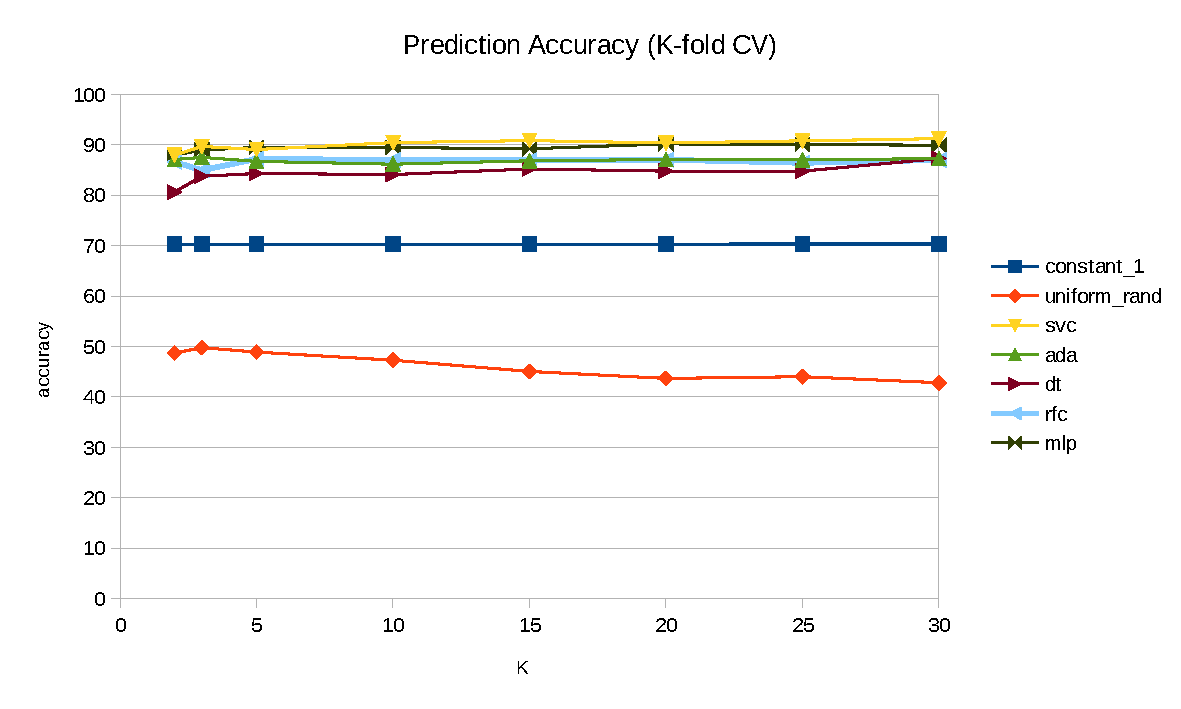
\includegraphics[width=0.45\textwidth]{figures/prediction_accuracy_kfold}
\caption{Prediction accuracy measured using k-fold CV on the whole SNU NPB loop set}
\label{fig:accuracy_kfold}
\end{figure}
%\begin{comment}
%\begin{table}[h!]
%    \centering
%    \begin{tabular}[c]{|p{1.5cm}|p{1.5cm}|p{1.5cm}|p{1.5cm}|}
%        \hline
%        ML model & accuracy & recall & precision \\
%        \hline
%        constant & 70.32 & 100 & 70.32\\
%        \hline
%        uniform & 46.27 & 41.50 & 69.79\\
%        \hline
%        SVC & 90.04 & 95.24 & 91.06 \\
%        \hline
%        AdaBoost & 86.96 & 92.92 & 89.06 \\
%        \hline
%        DT & 84.36 & 89.57 & 87.90 \\
%        \hline
%        RFC & 86.65 & 93.22 & 88.47 \\
%        \hline
%        MLP & 89.40 & 93.77 & 91.39 \\
%        \hline
%    \end{tabular}
%    \caption{Average predictive performance for different ML models measured %with a k-fold CV method on the whole set of 1415 SNU NPB loops.}
%    \label{tab:average_accuracy}
%\end{table}
%\end{comment}
\begin{table}
  \begin{minipage}{\columnwidth}
  \begin{center}
    \begin{tabu}{cccc}
      \hline
      \rowfont{\bfseries}
      ML model & accuracy & recall & precision\\\hline
      constant & 70.32 & 100 & 70.32\\
      uniform & 46.27 & 41.50 & 69.79\\
      SVC & 90.04 & 95.24 & 91.06 \\
      AdaBoost & 86.96 & 92.92 & 89.06 \\
      DT & 84.36 & 89.57 & 87.90 \\
      RFC & 86.65 & 93.22 & 88.47 \\
      MLP & 89.40 & 93.77 & 91.39 \\\hline
      \end{tabu}
  \end{center}
  \end{minipage}
  \caption{Average predictive performance for different ML models measured with a K-fold CV method on the whole set of 1415 SNU NPB loops.} 
  \label{tab:average_accuracy_models}
\end{table}%

\quad Table \ref{tab:average_accuracy} shows the average predictive performance for different ML models. The Support Vector Classifier (SVC) model has the highest accuracy and has successfully managed to recall 95,25\% of all parallel loops. ICC succeeds to parallelise 812 out of 995 parallelisable loops. SVC extends ICC parallelisation capabilities to 945 loops. Despite relatively high precision of 91.06\%, that extension comes at the price of some misprediction errors. Figure \ref{fig:prediction_stats} shows that unsafe (false positive) mispredictions dominate at 65.47\% of those cases where misclassification occurs. 
%Thus we need to devise a scheme, that will protect us and make these errors not that critical.

\begin{figure}[ht]
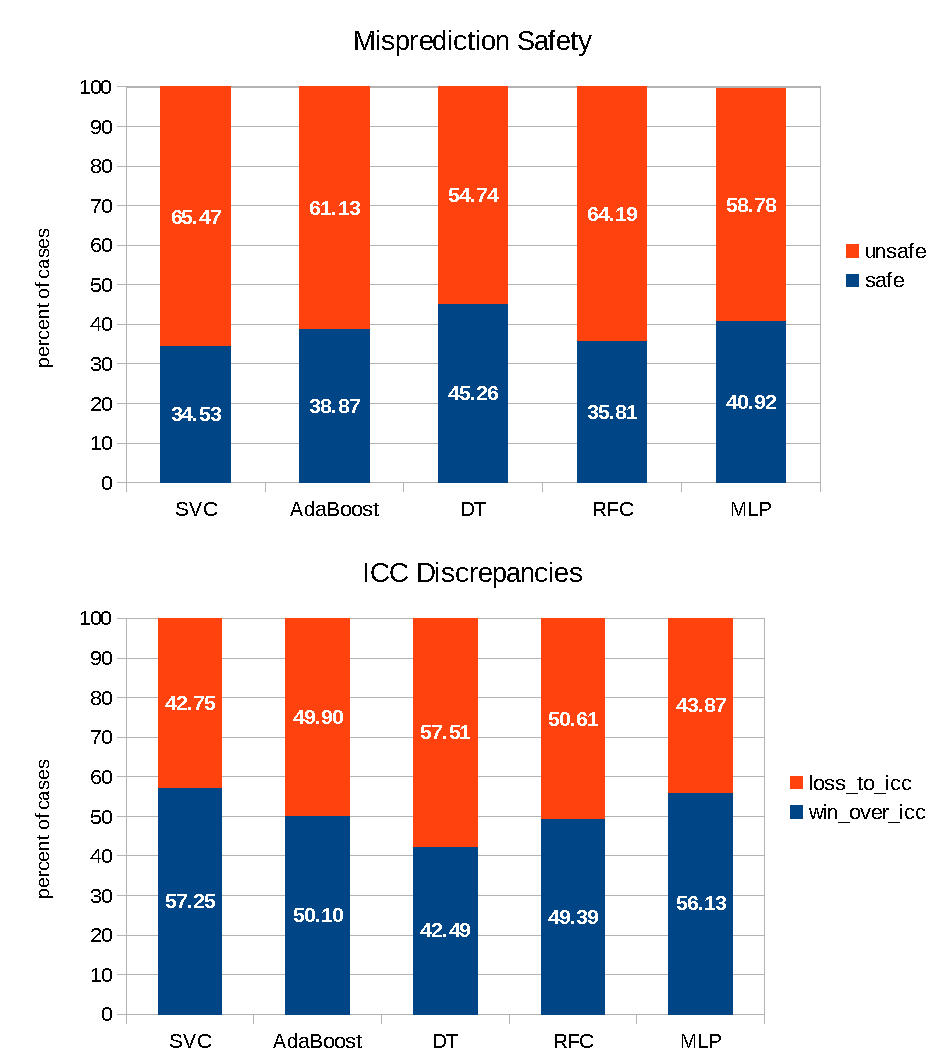
\includegraphics[width=0.45\textwidth]{figures/prediction_stats.pdf}
\caption{Breakdown of misclassification errors.}
\label{fig:prediction_stats}
\end{figure}

\subsection{LOOCV SNU NAS Performance}
\label{evaluation_loocv}

Next we perform a cross-validation experiment using  Leave-One-Out cross-validation (LOOCV). Instead of treating the entire set of loops from all benchmarks applications as a single data set, we now train our model on 9 benchmarks and test it on the remaining one. Doing so allows us to actually parallelise predicted parallel loops and to obtain parallel performance figures for the benchmark application under consideration.

%\quad While k-fold cross-validation method mixes loops from all 10 SNU NPB benchmarks and provides a good statistical assessment of predictive performance on the whole SNU NPB data set generally, in order to use our predictor with the proposed schemes we need to change our methodology. For that purpose we use modified Leave-One-Out cross-validation (LOOCV) technique. We train our model on 9 benchmarks and test it on the remaining one. Doing so allows us to actually parallelise all correctly predicted parallel loops and get performance numbers for the benchmark being tested.
%\begin{comment}
%\begin{table*}[t!]
%    \centering
%    \begin{tabular}[c]{|p{1.5cm}|p{1.0cm}|p{1.5cm}|p{1.3cm}|p{1.0cm}|p{1.5cm}|%p{1.3cm}|p{1.0cm}|p{1.5cm}|p{1.3cm}|}
%        \hline
%        benchmark & \multicolumn{3}{c}{average per model} \vline &	%\multicolumn{3}{c}{most frequent} \vline & \multicolumn{3}{c}{uniform} \vline %\\
%        \hline
%	    accuracy & recall &	precision &	accuracy & recall &	precision &	%accuracy &	recall	& precision & accuracy \\
%	    \hline
%        BT & 85.7 & 92.6 & 90.0 & 78.4 & 100.0 & 78.4 & 51.9 & 48.3 & 83.3 \\
%        \hline
%        CG & 74.2 & 72.4 & 85.7	& 64.4 & 100.0 & 64.4 & 46.7 & 37.9 & 64.7 %\\
%        \hline
%        DC & 72.8 & 71.0 & 51.5	& 29.0 & 100.0 & 29.0 & 55.0 & 37.9 & 28.9 %\\
%        \hline
%        EP & 92.0 &	86.6 & 100.0 & 60.0 & 100.0 & 60.0 & 40.0 & 33.3 & 50.0 %\\
%        \hline
%        FT & 56.5 &	37.9 & 84.4	& 63.0 & 100.0 & 63.0 & 43.5 & 34.5	& 58.8 %\\
%        \hline
%        IS & 74.0 &	97.5 & 61.3	& 40.0 & 100.0 & 40.0 &	45.0 & 37.5	& 33.3 %\\
%        \hline
%        LU & 90.1 &	90.7 & 96.3	& 78.0 & 100.0 & 78.0 & 46.1 & 45.0	& 76.1 %\\
%        \hline
%        MG & 64.9 &	87.6 & 57.8	& 45.7 & 100.0 & 45.7 &	43.2 & 32.4	& 36.4 %\\
%        \hline
%        SP & 88.8 &	94.7 & 92.2	& 83.4 & 100.0 & 83.4 &	46.6 & 46.4	& 81.7 %\\
%        \hline
%        UA & 75.9 &	83.8 & 83.9	& 72.9 & 100.0 & 72.9 &	48.4 & 47.2	& 72.5 %\\
%        \hline
%    \end{tabular}
%    \caption{Predictive performance on different for different ML models %measured with a k-fold CV method on the whole set of 1415 SNU NPB loops.}
%    \label{tab:average_accuracy}
%\end{table*}
%\end{comment}

\begin{table*}
  \begin{minipage}{\textwidth}
  \begin{center}
    \begin{tabu}{c|ccc|ccc|ccc}
      \hline
      \rowfont{\bfseries}
      Benchmark & \multicolumn{3}{c}{Average Per Model} \vline & \multicolumn{3}{c}{Most Frequent} \vline & \multicolumn{3}{c}{Uniform}\\\hline
      \rowfont{\bfseries}
      Accuracy & Recall & Precision & Accuracy & Recall & Precision & Accuracy & Recall	& Precision & Accuracy\\\hline
      BT & 85.7 & 92.6 & 90.0 & 78.4 & 100.0 & 78.4 & 51.9 & 48.3 & 83.3 \\
      CG & 74.2 & 72.4 & 85.7	& 64.4 & 100.0 & 64.4 & 46.7 & 37.9 & 64.7 \\
      DC & 72.8 & 71.0 & 51.5	& 29.0 & 100.0 & 29.0 & 55.0 & 37.9 & 28.9 \\
      EP & 92.0 &	86.6 & 100.0 & 60.0 & 100.0 & 60.0 & 40.0 & 33.3 & 50.0 \\
      FT & 56.5 &	37.9 & 84.4	& 63.0 & 100.0 & 63.0 & 43.5 & 34.5	& 58.8 \\
      IS & 74.0 &	97.5 & 61.3	& 40.0 & 100.0 & 40.0 &	45.0 & 37.5	& 33.3 \\
      LU & 90.1 &	90.7 & 96.3	& 78.0 & 100.0 & 78.0 & 46.1 & 45.0	& 76.1 \\
      MG & 64.9 &	87.6 & 57.8	& 45.7 & 100.0 & 45.7 &	43.2 & 32.4	& 36.4 \\
      SP & 88.8 &	94.7 & 92.2	& 83.4 & 100.0 & 83.4 &	46.6 & 46.4	& 81.7 \\
      UA & 75.9 &	83.8 & 83.9	& 72.9 & 100.0 & 72.9 &	48.4 & 47.2	& 72.5 \\\hline
      \end{tabu}
  \end{center}
  \end{minipage}
  \caption{Average predictive performance for different ML models measured with a K-fold CV method on the whole set of 1415 SNU NPB loops.} 
  \label{tab:average_accuracy_kfold}
\end{table*}%


\begin{figure}[ht]
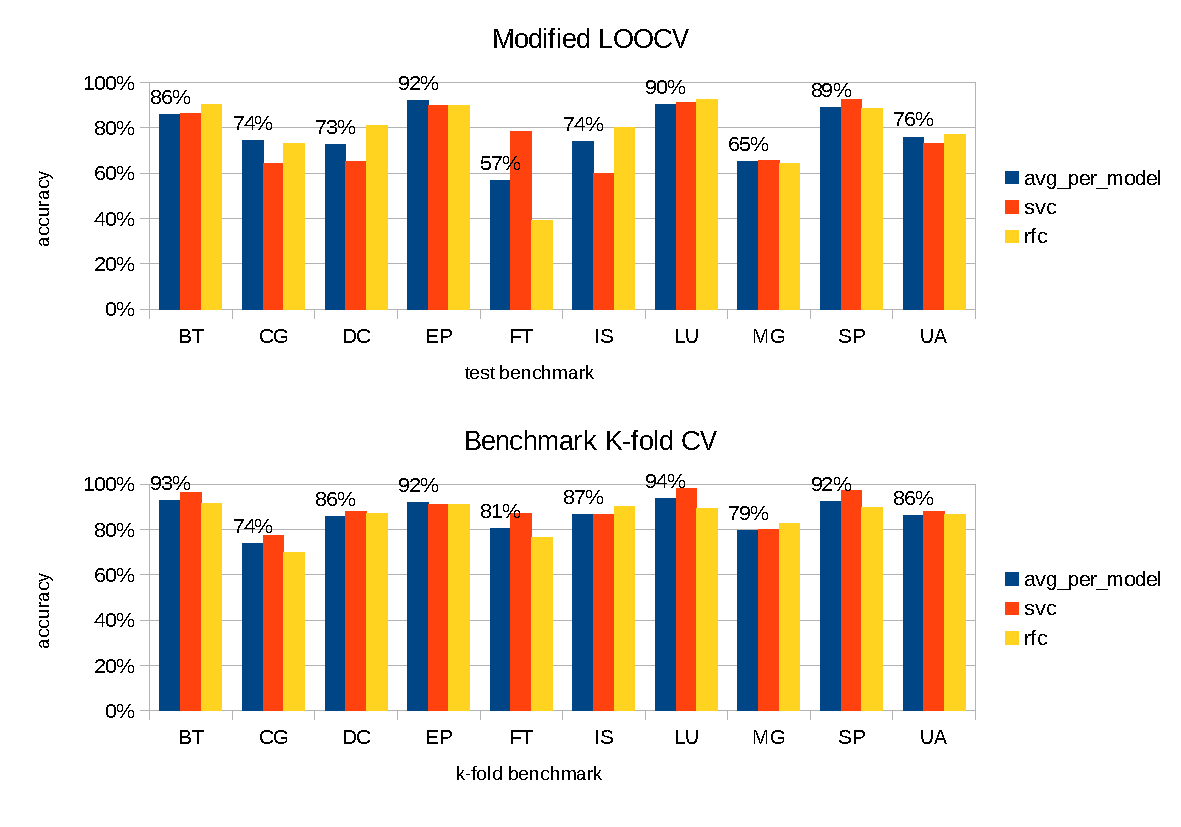
\includegraphics[width=0.45\textwidth]{figures/LOOCV_accuracy.pdf}
\caption{Prediction accuracy measured using k-fold CV on the entire SNU NPB loop set.}
\label{fig:accuracy_loocv}
\end{figure}

\section{Parallelization Assistant}
\label{practical_applications}

The ML-based predictor developed in the previous two sections is a core component of our novel parallelisation assistant. This assistant incorporates prediction results on whether a loop can be parallelised and combines this with profiling information. It then produces a ranking of all loops in an application to guide the programmer towards the most beneficial loop candidates for their \textit{manual} parallelisation effort. We do not seek to replace the human parallelisation expert from the process, but aim to assist the programmer and increase their productivity.

%\quad Achieving high predictive performance is not enough. We need to find a real practical application of our loop parallelisability predictor. Due to statistical nature inherent to all machine learning techniques it is impossible to eliminate all prediction errors completely. While false negative mispredictions might just miss available parallelisation opportunities and lose some performance, false positive mispredictions can break the program and are the most critical in the context of our ML problem.
%\paragraph{\textbf{Loop Parallelisation Assistant}} Taking the above mentioned fact into consideration we propose to integrate our trained predictor into an assistant scheme, which leaves the final parallelisation decision up to a programmer. Taking application profile as an input our assistant computes a ranking score for every loop in the application. 

\paragraph{Loop Ranking.}
The loop ranking computed by our parallelisation assistant combines a loop's contribution to overall execution time as well as its predicted likelihood of being parallelisable. In particular, we obtain the ranking by applying a shifted sigmoid function to the predicted parallelisability likelihood multiplied by the loop runtime as shown in Figure \ref{fig:sigmoid_3d}.
\begin{figure}[ht]
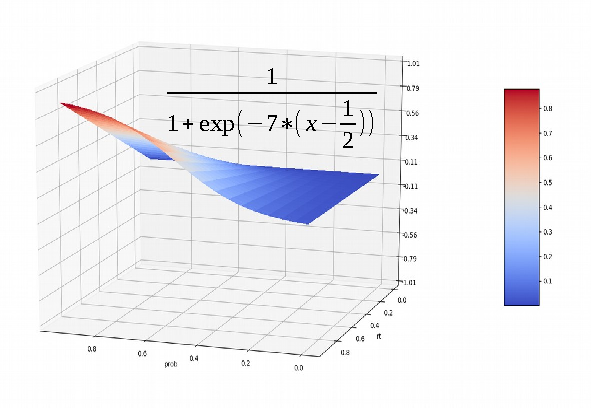
\includegraphics[width=0.45\textwidth]{figures/sigmoid_3d.pdf}
\caption{The ranking function combines for each loop its contribution to an application's overall execution time and its predicted likelihood of being parallelisable.}
\label{fig:sigmoid_3d}
\end{figure}

The intuition for using this function to combine the two metrics is that it prioritises parallelisable long-running loops and scales down the weight of non-parallelisable loops irrespective of their contribution to execution time. The effect of this can be seen in Figure \ref{fig:ft_loop_ranking} for the loops of the FT benchmark.

%With a more detailed examination it is visible, that the shape of the function is chosen in a way, that it ranks parallelisable long-running program loops the highest and tries to amplify all non-parallelisable loops down irrespective of their running time. The effect is better demonstrated with the case study presented on the figure \ref{fig:ft_loop_ranking}, which highlights the contrast between different rankings of FT benchmark loops.

\begin{figure*}[!ht]
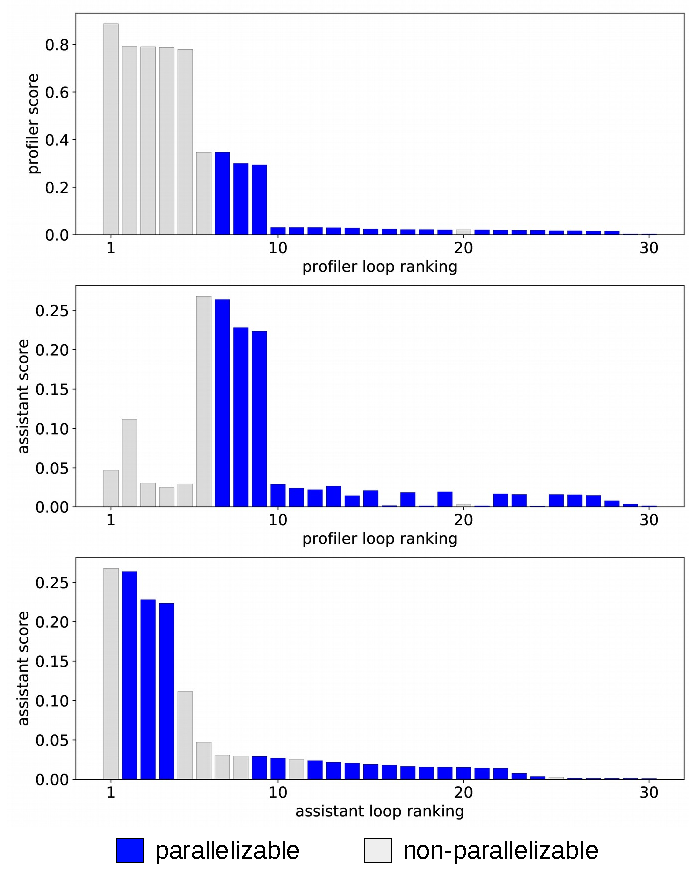
\includegraphics[width=\textwidth]{figures/ft_filter.pdf}
\caption{Change of loop rankings after the application of the ranking function for the 46 loops of SNU NPB FT benchmark. Where scoring based on loop execution time alone (top left) results in some high-ranked, but non-parallelisable loops (top right), combining profiled execution time and predictability in the score (bottom left) results in a ranking that prioritises parallel loop candidates (bottom right).}
\label{fig:ft_loop_ranking}
\end{figure*}

If programmers attempt to parallelise loops in the order prescribed by their execution time, they will inevitably waste their time trying to parallelise loops which may be long-running, but offer little or no opportunity for extracting parallelism. Instead, when combined in a ranking including predicted parallelisation success the new ranking directly guides the programmer to those loops, which significantly contribute to overall execution time \textbf{and} offer a reaslistic prospect of parallelisation.

%Top left and right pictures are identical and rank FT benchmark loops according to their running time score (given by the Intel Compiler). The problem with that order is that it ranks long-running program loops the highest independent of their parallelisability. If a programmer starts to parallelise application following that order, he is going to waste his time and efforts on the loops one cannot parallelise anyway. The left and right plots at the bottom of the figure demonstrate a transformation in the loop ranking our assistant does. Vertical axes of these plots correspond to the values our shifted sigmoid ranking function (see figure \ref{fig:sigmoid_3d}) takes. The bottom left plot shows how the relative height of the bars changes with a switch from a loop runtime to our scoring function. It is clear from the plot, that non-parallelisable loops go down in their importance. The bottom right picture shows that such a change actually moves true parallel loops toward the beginning of the list. The longer loop takes to run, the bigger the move. On the other hand non-parallelisable loops move towards the back of the list (almost independent of their running time). The improved ranking of FT loops allows a programmer to immediately start benchmark parallelisation with the most important loops and don't waste time looking at long-running loops, which cannot be parallelised by their nature anyway.
\begin{comment}
\begin{figure}[ht]
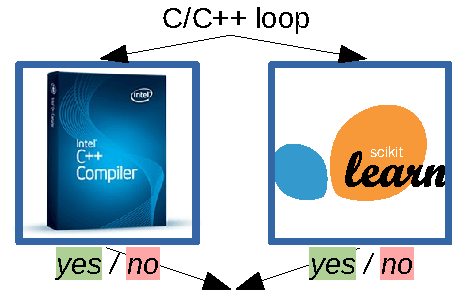
\includegraphics[width=0.45\textwidth]{figures/icc_competition_scheme.pdf}
\caption{First predictor application. Smart parallelisation adviser. }
\label{fig:icc_competition_scheme}
\end{figure}
\end{comment}

\subsection{Comparison to Static Analysis} 

We have compared the generated rankings of our parallelisation assistant with the Intel \cpp{} Compiler, which due to its use of static analysis is conservative and occasionally misses some parallelisation opportunities.

\begin{comment}
\begin{table}[ht]
    \centering
    \begin{tabular}[c]{|p{1.0cm}|p{1.5cm}|p{1.5cm}|p{2cm}|}
        \hline
        ICC & predictor & true parallel & classification bucket \\
        \hline
        0 & 0 & 0 & correct 0 (no) prediction \\
        \hline
        0 & 0 & 1 & missed opportunity \\
        \hline
        0 & 1 & 0 & false positive \\
        \hline
        0 & 1 & 1 & discovery \\        
        \hline
        1 & 0 & 0 & impossible \\
        \hline
        1 & 0 & 1 & icc shielding \\
        \hline
        1 & 1 & 0 & impossible \\
        \hline
        1 & 1 & 1 & correct 1 (yes) prediction \\  
        \hline
    \end{tabular}
    \caption{All the possible ICC competition scheme combinations}
    \label{tab:combinations_table}
\end{table}
\end{comment}
\begin{table}
  \begin{minipage}{\columnwidth}
  \begin{center}
    \begin{tabu}{M{0.5cm}M{1.2cm}M{2.0cm}M{3.5cm}}
      \hline
      \rowfont{\bfseries}
      ICC & Predictor & True Parallel & Classification Bucket\\%\hline
      \hline
      0 & 0 & 0 & correct 0 (no) prediction\\
      0 & 0 & 1 & missed opportunity\\
      0 & 1 & 0 & false positive\\
      0 & 1 & 1 & discovery\\
      1 & 0 & 0 & impossible\\
      1 & 0 & 1 & icc shielding\\
      1 & 1 & 0 & impossible\\
      1 & 1 & 1 & correct 1 (yes) prediction\\\hline  
    \end{tabu}
  \end{center}
  \end{minipage}
  \caption{Possible outcomes for the side-by-side setup of our ML predictor and Intel's parallelising compiler.}
  \label{tab:combinations_table}
\end{table}%

The ML approach to parallelisation with a human expert responsible for final code transformation allows our parallelisation assistant to be more aggressive than ICC. Hence, our model can predict more loops as parallelisable than ICC. The visible effect of this is that our assistant potentially assigns high probabilities to some possibly-parallel loops and awards them a relatively high rank, despite the fact that ICC is not capable of parallelising them. In Table \ref{tab:combinations_table} these loops are classified under ``discovery".

We have set up an experiment where we apply our ML predictor side-by-side with ICC.  Both aim at independently classifyings loops as parallelisable or not. There are a total of 6 possible classification outcomes our scheme might potentially produce summarised in Table \ref{tab:combinations_table}. The most interesting cases are those, where the ML predictor disagrees with ICC. We then manually inspected these cases and investigated the cause of conservatism in ICC. 

A summary and breakdown by reason for ICC's failure to parallelise a loop can be found in Table \ref{tab:icc_missed_opportunities}.
\begin{table}
  \begin{minipage}{\columnwidth}
  \begin{center}
    \begin{tabu}{M{1.6cm}M{0.5cm}M{1.6cm}M{0.5cm}M{1.6cm}M{0.5cm}}
      \hline
      \rowfont{\bfseries}
      reason & num & reason & num & reason & num\\\hline
      \textbf{unrecognised reduction} & 18 & \textbf{array privatization} & 7 & \textbf{AA conservativeness} & 60\\\hline
      \textbf{unknown iteration number} & 7 & \textbf{static dependencies} & 46 & \textbf{too complex} & 22\\\hline
      \textbf{uninlined calls} & 4 & \textbf{other} & 4 & \textbf{total} & 168\\\hline
    \end{tabu}
  \end{center}
  \end{minipage}
  \caption{Classification of parallelisable loops rejected for parallelisation by Intel's compiler.}
  \label{tab:icc_missed_opportunities}
\end{table}%

\subsection{Classification Performance}
\label{evaluation_icc_competition}

Next we evaluate the classification performance and misclassifications according to Table \ref{tab:combinations_table}. We repeatedly ran K-fold CV on the whole set of SNU NPB loops and sorted the outcomes into separate buckets.
Figure \ref{fig:icc_competition} shows the final distribution of all the cases as percentages of the total number of bucket classifications. In majority of cases our parallelisation assistant agrees with ICC and either classifies truly non-parallel loops as non-parallel or truly parallel loops as parallel. This is an expected results as we have used ICC (along with OpenMP annotated loops) to train our ML model. However, sometimes our parallelisation assistant and ICC reached different conclusions. The results are shown in Figure \ref{fig:icc_competition}. As can be seen differences are mainly due to our parallelisation assistant discovering parallelisable loops inaccessible to ICC, but also due to small proportion of false positives.

\begin{figure}[t!]
\begin{minipage}{\columnwidth}
\centering
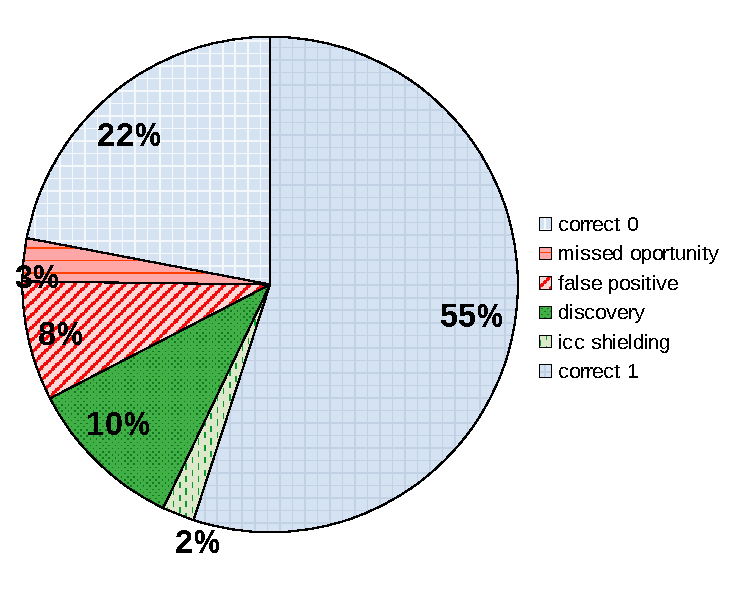
\includegraphics[width=\columnwidth]{figures/icc_vs_predictor.pdf}
\caption{Intel Compiler (ICC) vs. Predictor. Distribution of different classification cases. By large our predictor agrees with ICC (80\%). In 8\% of cases  }
\label{fig:icc_competition}
\end{minipage}
\end{figure}


\begin{figure*}[t!]
\centering
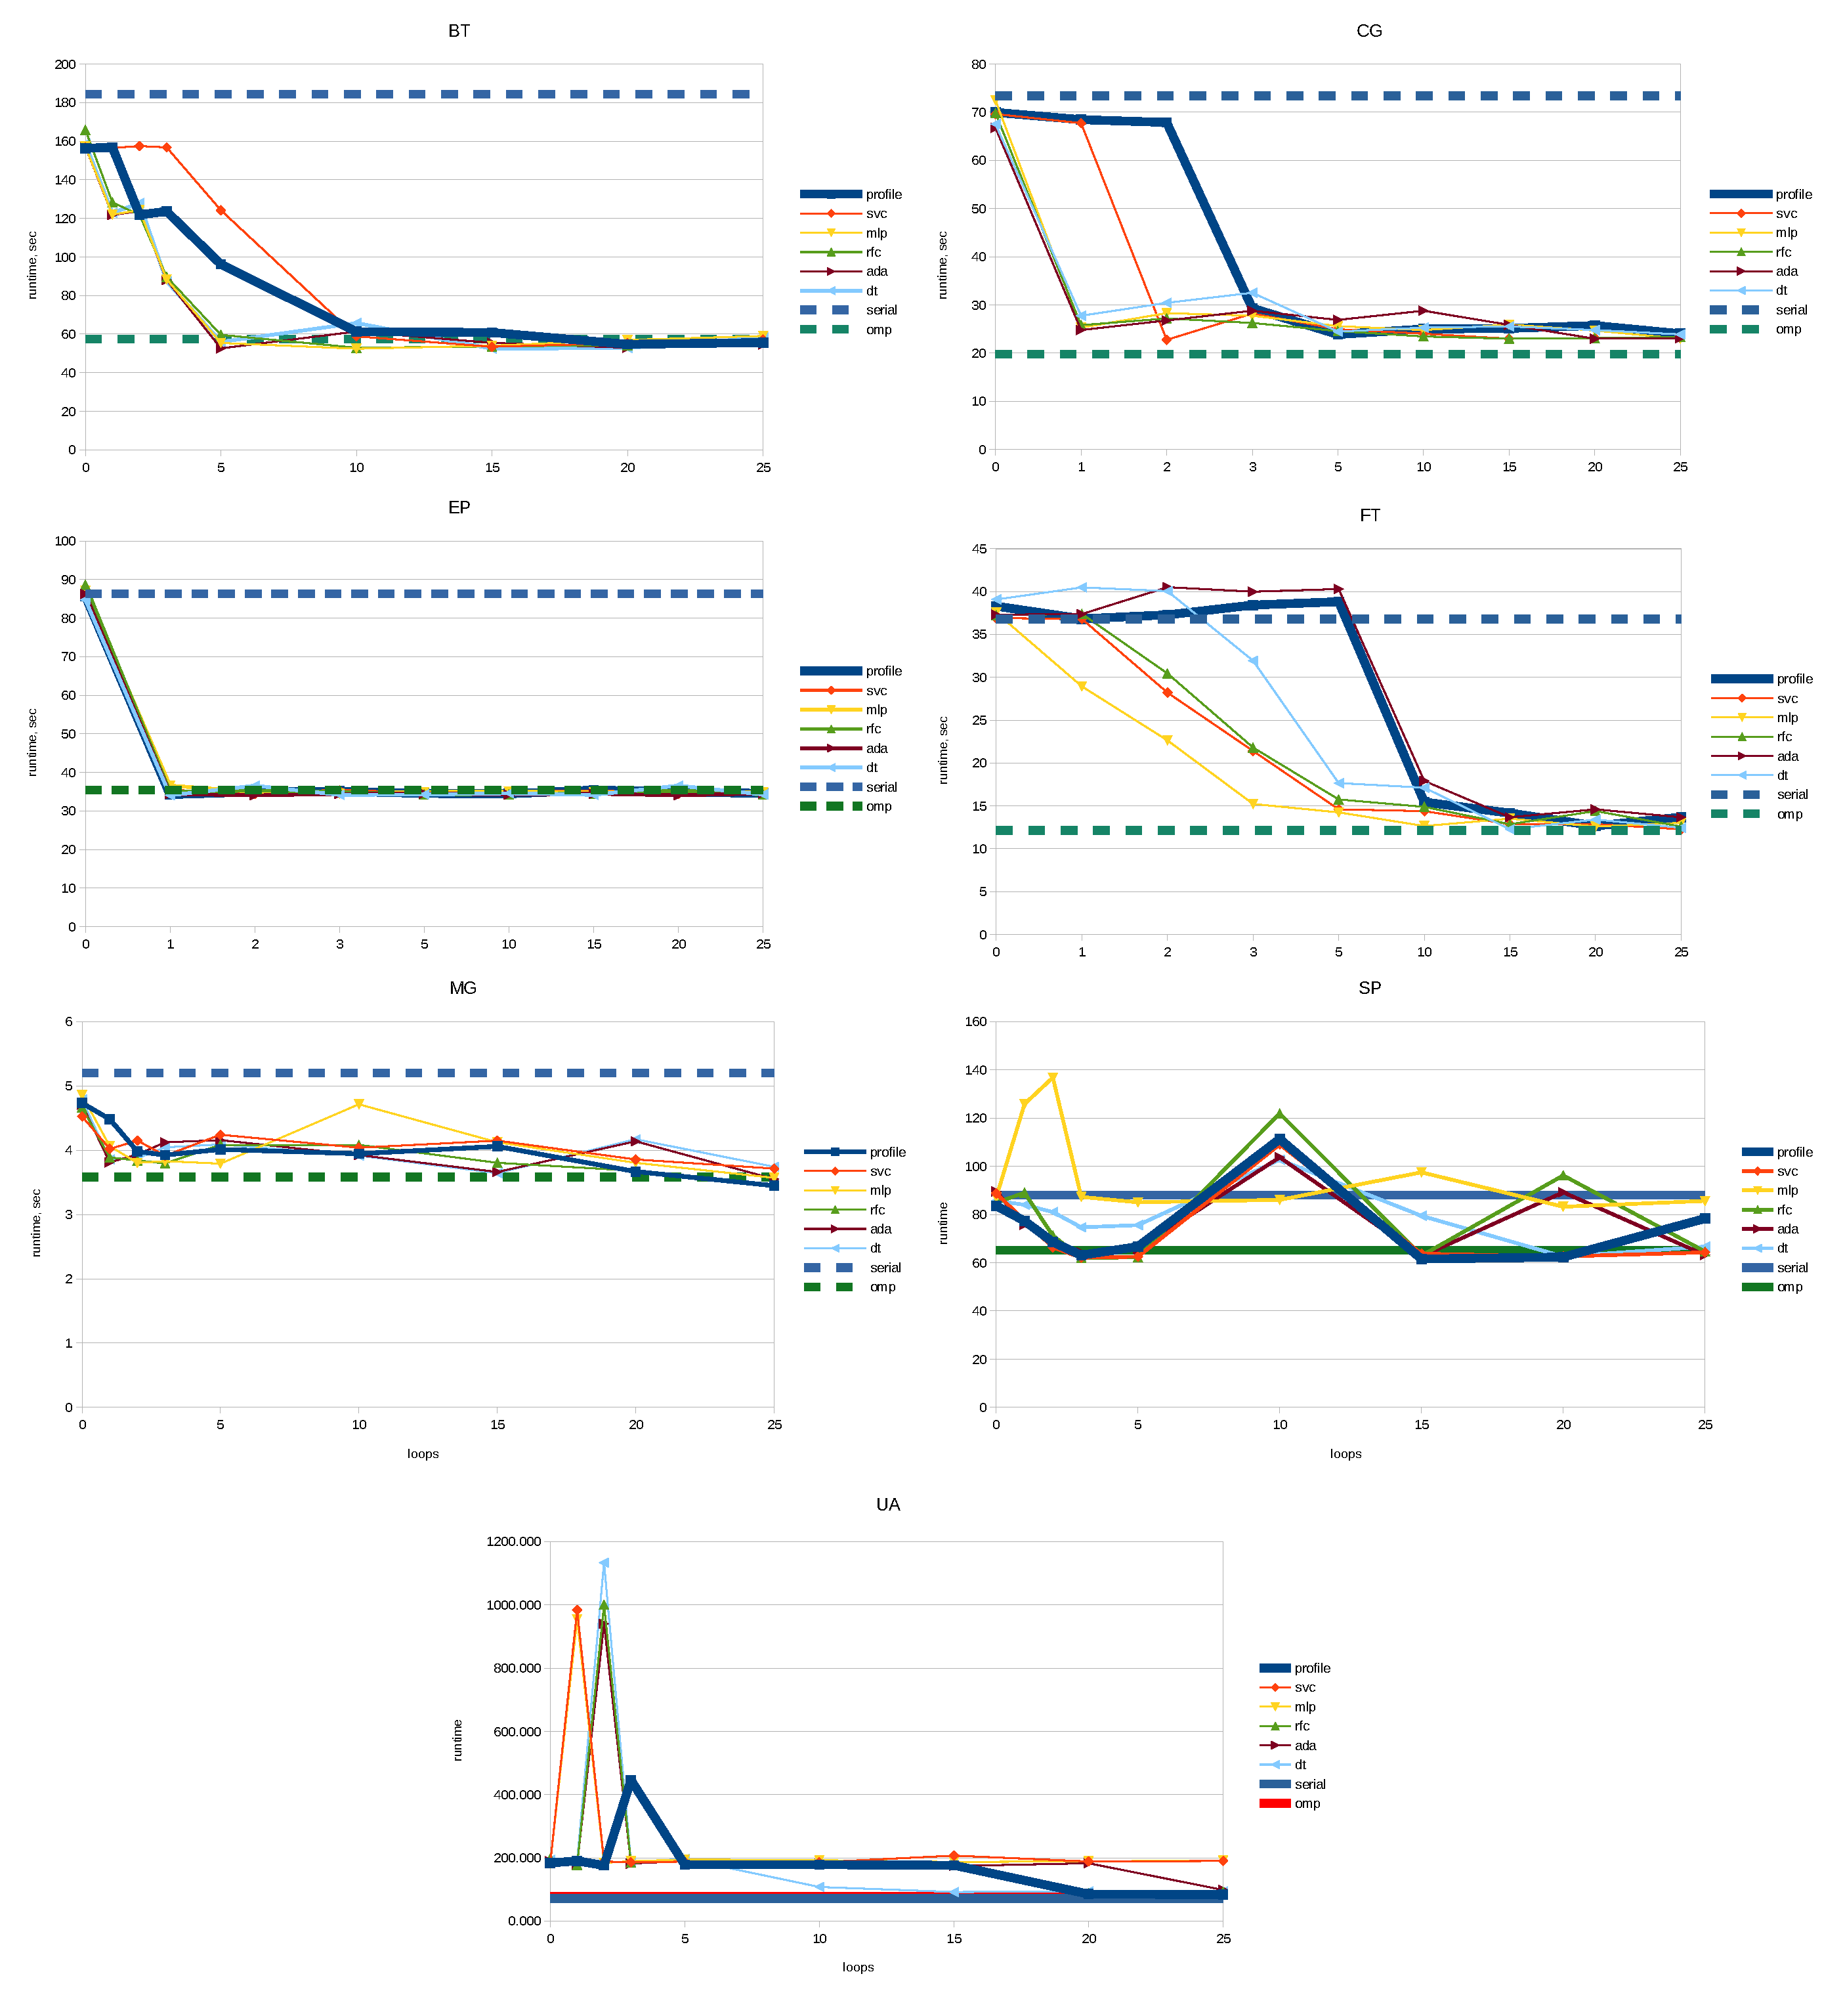
\includegraphics[width=0.95\textwidth]{figures/perf_conv_curves.pdf}
\caption{From left to right more loops are parallelised for each benchmark. As we parallelise more loops, program execution times improve over the initial sequential performance and reach the performance level of the reference OpenMP implementations. Our ML based parallelisation assistant requires the user to parallelise fewer loops than a purely profile-guided approach to reach maximum parallel speedup.}
\label{fig:performance_convergence_line}
\end{figure*}

\section{End-to-End Evaluation}
\label{evaluation}

In this section we evaluate the performance of our parallelisation assistant. In particular, we are interested in the potential productivity gains delivered by our parallelisation assistant and savings on human expert time.

In our study we assume the human expert to start with sequential C implementations of the SNU NAS benchmarks. The goal is to parallelise these benchmark applications to a standard and performance level to that of the (existing) parallel versions of the benchmark. By using our parallelisation assistant we expect the human expert to consider fewer loops than by following a profiling-based approach, i.e.\ considering loops in the order of decreasing contributions to overall program execution time. We also compare against the fully automated parallelisation approach implemented in the ICC compiler.

Our results are shown as performance convergence curves in Figure \ref{fig:performance_convergence_line}. For each benchmark we present the execution time (on the y-axis) in dependence on the number of parallelised loops (on the x-axis). Execution time is bounded to the top by the original sequential execution time, and to the bottom by the time for the reference OpenMP implementation written by human experts.

We notice that the Intel compiler not only fails to achieve noticeable speedups, but actually slows the performance down on most of the benchmarks. For BT benchmark the slowdown reaches 3,5 times. In contrast, the reference OpenMP implementation results in a (geo-)mean speedup of 2.19 across the benchmark suite. 

As seen in Figure \ref{fig:performance_convergence_line} our parallelisation assistant requires the user to parallelise significantly fewer loops than a profile-guided approach for the BT, CG, FT and UA benchmarks. For BT, maximum parallel performance is reached after the user has parallelised the first five loops suggested by the ranking of our parallelisation assistant, while profile-guided parallelisation requires about 20 loops to be parallelised to reach the same performance level. While there is some variation depending on the ML model used for the parallelisation prediction, in general ML assisted parallelisation outperforms or equals the profile-guided schemes in all benchmarks. In several cases (BT, CG, FT) the parallelisation assistant enables the user to reach the parallel performance maximum much earlier than the profile-guided scheme, thus demonstrating the effectiveness of our tool and methodology.

However, we also observe that our parallelisation adviser does not reach the performance of the reference OpenMP versions on the DC and IS benchmarks. Manual inspection reveals that these benchmarks have been parallised using OpenMP parallel sections, but do not contain any OpenMP parallel loops. Our parallelisation assistant incorrectly suggest to parallelise some of the benchmark loops, though. Table \ref{tab:average_accuracy} summarises the outcomes of the application of our parallelisation assistant on the NPB NAS benchmarks.

%are actually demonstrating the deployment of our assistant on SNU NAS Parallel Benchmarks. But before we can assess our assistant we need to conduct a study of performance one could potentially extract from SNU NPB benchmarks. Having measured running times of differently compiled versions, we discovered that ICC compiler not only fails to achieve noticeable speedups, but actually slows the performance down on most of the benchmarks. For BT benchmark the slowdown is striking 3,5 times. Manual expertly done OpenMP parallelisation of SNU NPB developers results into the geomean speedup of 2.19x.\newline\null

%\quad To conduct SNU NPB assistant deployment experiment we had to use a modified LOOCV. For every single SNU NPB benchmark we used the 9 remaining ones to train the predictor and get the ranking of benchmark loops. As section \label{loocv_accuracy} shows such a methodology has a lower predictive performance due to training set incompleteness, which potentially limits the success of our technique. After that we followed the ranking and parallelised the chosen benchmark loop by loop until we managed to achieve the performance level of an expertly parallelised version. We repeated the process for different ML models as well as for a profile based ranking and plotted the performance convergence curves on figure \ref{fig:performance_convergence_line}. Our technique is not applicable to DC and IS benchmarks: these benchmarks get their parallel speedups from OpenMP parallel sections and not from parallel loops. Parallelisation of loops in these benchmarks (be it profile ordered list or the one of our adviser) actually slows them down.  
%\begin{comment}
%\begin{figure*}[th]
%\centering
%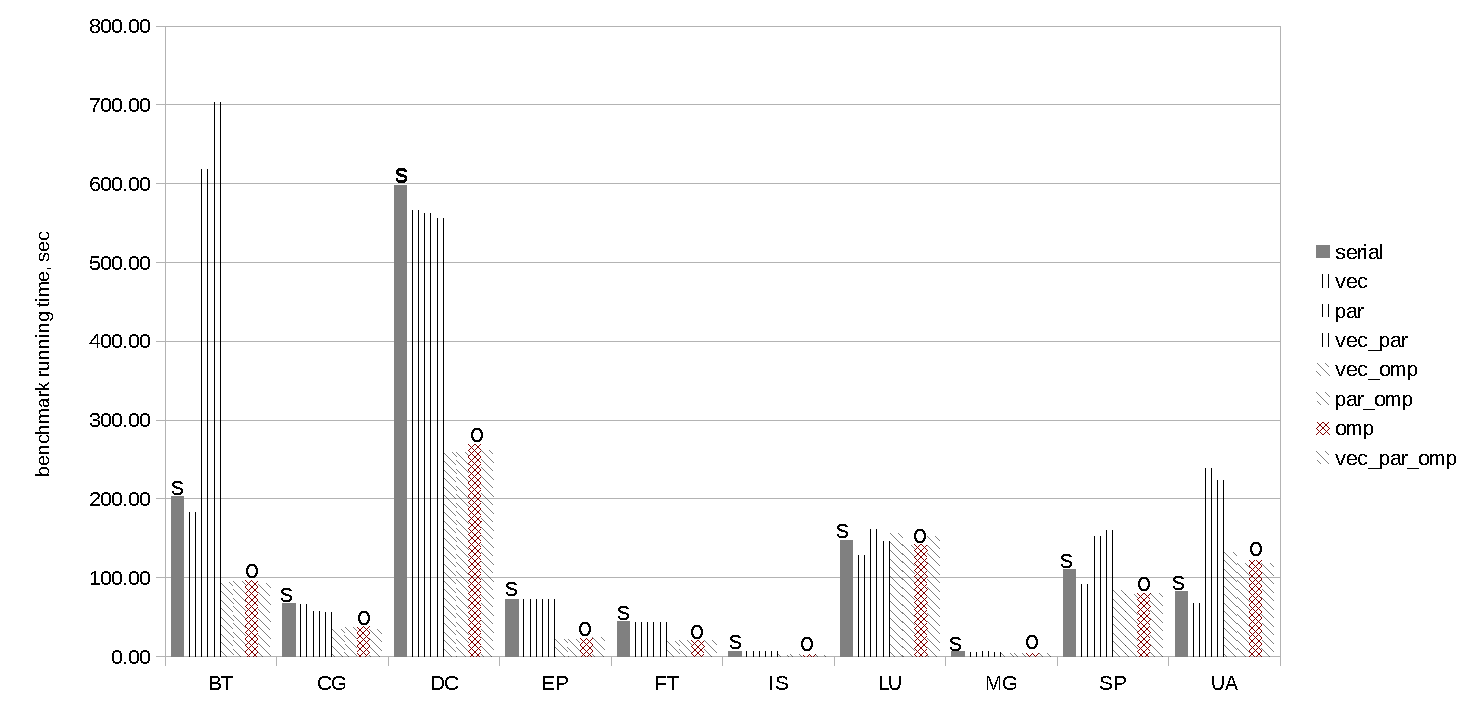
\includegraphics[width=\textwidth]{figures/benchmark_runtime.pdf}
%\caption{SNU NPB running times for different compilation options: serial, %automatic parallelisation and vectorization, OpenMP benchmark expert developer %version and all the possible combinations of those.}
%\label{fig:snu_npb_performance}
%\end{figure*}
%\end{comment}




\begin{table*}
  \begin{minipage}{\textwidth}
  \begin{center}
    \begin{tabu}{c|ccc|cc|c|ccccc}
      \hline
      \rowfont{\bfseries}
      \multirow{2}{*}{Benchmark} & \multicolumn{3}{c}{Benchmark Runtime, \textit{sec}} \vline & \multicolumn{2}{c}{Speedup, \textit{times}} \vline & \multicolumn{6}{c}{$Loops\ Number_{LOC}$}\\\cline{2-12}
      \rowfont{\bfseries}
      & Serial & OpenMP & Critical & OpenMP & Critical & Profile & SVC & MLP & RFC & AdaBoost & DT\\\hline
      BT & 158.76 & 57.36 & 56.57 & 2.77 & 2.81 & $6_\textit{6122}$ & \cellcolor[HTML]{FA8D8D} $8_\textit{6392}$ & \cellcolor[HTML]{7BB66B} $4_\textit{4088}$ & \cellcolor[HTML]{7BB66B} $5_\textit{5105}$ & \cellcolor[HTML]{7BB66B} $3_\textit{3061}$ & \cellcolor[HTML]{7BB66B} $5_\textit{5105}$\\
      CG & 69.38 & 19.77 & 25.06 & 3.51 & 2.77 & $3_\textit{330}$ & \cellcolor[HTML]{7BB66B} $2_\textit{118}$ & \cellcolor[HTML]{7BB66B} $1_\textit{6}$ & \cellcolor[HTML]{7BB66B} $1_\textit{6}$ & \cellcolor[HTML]{7BB66B} $1_\textit{6}$ & \cellcolor[HTML]{7BB66B} $1_\textit{6}$\\
      DC & 698.82 & 254.29 & 698.82 & 2.75 & 1.00 & $\infty$ & \cellcolor[HTML]{91A1FA} $\infty$ & \cellcolor[HTML]{91A1FA} $\infty$ & \cellcolor[HTML]{91A1FA} $\infty$ & \cellcolor[HTML]{91A1FA} $\infty$ & \cellcolor[HTML]{91A1FA} $\infty$\\
      EP & 86.35 & 35.40 & 35.07 & 2.44 & 2.46 & $1_\textit{45}$ & \cellcolor[HTML]{91A1FA} $1_\textit{45}$ & \cellcolor[HTML]{91A1FA}$1_\textit{45}$ & \cellcolor[HTML]{91A1FA} $1_\textit{45}$ & \cellcolor[HTML]{91A1FA} $1_\textit{45}$ & \cellcolor[HTML]{91A1FA} $1_\textit{45}$\\
      FT & 36.81 & 12.13 & 14.69 & 3.03 & 2.51 & $9_\textit{338}$ & \cellcolor[HTML]{7BB66B} $4_\textit{187}$ & \cellcolor[HTML]{7BB66B} $3_\textit{140}$ & \cellcolor[HTML]{7BB66B} $4_\textit{187}$ & \cellcolor[HTML]{91A1FA} $9_\textit{338}$ & \cellcolor[HTML]{7BB66B} $5_\textit{193}$\\
      IS & 4.75 & 1.35 & 4.63 & 3.53 & 1.03 & $\infty$ & \cellcolor[HTML]{91A1FA} $\infty$ & \cellcolor[HTML]{91A1FA} $\infty$ & \cellcolor[HTML]{91A1FA} $\infty$ & \cellcolor[HTML]{91A1FA} $\infty$ & \cellcolor[HTML]{91A1FA} $\infty$\\
      LU & 115.46 & 55.00 & 140.53 & 2.10 & 0.82 & $\infty$ & \cellcolor[HTML]{91A1FA} $\infty$ & \cellcolor[HTML]{91A1FA} $\infty$ & \cellcolor[HTML]{91A1FA} $\infty$ & \cellcolor[HTML]{91A1FA} $\infty$ & \cellcolor[HTML]{91A1FA} $\infty$\\
      MG & 5.20 & 3.58 & 3.94 & 1.45 & 1.32 & $3_\textit{43}$ & \cellcolor[HTML]{91A1FA} $3_\textit{43}$ & \cellcolor[HTML]{91A1FA} $3_\textit{43}$ & \cellcolor[HTML]{91A1FA} $3_\textit{43}$ & \cellcolor[HTML]{91A1FA} $3_\textit{43}$ & \cellcolor[HTML]{91A1FA} $3_\textit{43}$\\
      SP & 86.65 & 65.19 & 62.90 & 1.33 & 1.38 & $3_\textit{801}$ & \cellcolor[HTML]{91A1FA} $3_\textit{801}$ & \cellcolor[HTML]{FA8D8D} $\infty$ & \cellcolor[HTML]{91A1FA} $3_\textit{801}$ & \cellcolor[HTML]{91A1FA} $3_\textit{801}$ & \cellcolor[HTML]{FA8D8D} $20_\textit{1257}$\\
      UA & 71.82 & 78.56 & 189.66 & 0.91 & 0.38 & $19_\textit{882}$ & \cellcolor[HTML]{FA8D8D} $30_\textit{918}$ & \cellcolor[HTML]{7BB66B} $30_\textit{508}$ & \cellcolor[HTML]{7BB66B} $19_\textit{861}$ & \cellcolor[HTML]{91A1FA} $22_\textit{883}$ & \cellcolor[HTML]{7BB66B} $10_\textit{579}$\\\hline
      \end{tabu}
  \end{center}
  \end{minipage}
  \caption{The final SNU NPB assistant deployment table. Columns show running times of all SNU NPB benchmarks for serial, fully parallelised OpenMP and partially parallelised (critical) versions. The partially parallelised versions have only several critical (top ranked) loops parallelised. The right hand part of the table shows the number of top-ranked loops one needs to parallelise in order to reach critical performance. In majority of cases ML based models converge to the critical performance faster than a profile based approach. Programmer efforts are approximated by the number of Lines Of Code (LOC) loops contain. The table shows that in order to fully parallelise SNU NPB suite to its critical performance using our assistant a programmer has to examine 20\% less LOC, then he would with a profiler only.} 
  \label{tab:average_accuracy}
\end{table*}%
%\begin{comment}
%\quad The common general thing about all SNU NAS benchmarks we observed is %that the main portion of benchmark speedup comes from a coarse-grain manual %parallelisation done by its developers. The main loops preceded by OpenMP %pragmas are quite big and complex. Usually they contain calls to different %%functions, which do not always get inlined, as well as a lot of %multidimensional arrays with complex index computations. Many array references %happen indirectly and thus require runtime behaviour knowledge for their %analysis. Parallelisation of such loops requires a thorough comprehension of %the source code by a programmer, and is beyond the capabilities of the %state-of-the-art automatic tools.\newline
%\quad Intel compiler vectorises and parallelises quite a significant number of %SNU NAS benchmark loops, but these loops are not the main ones. When we %measure the performance of parallel and vector codes generated by Intel %compiler, we observe running times being slightly better than in serial %versions for vector codes and significant slowdowns for automatic ICC %parallelisation.       
%\quad The major weakness of Intel compiler, as well as our trained loop %parallelisability classifier is that they mostly discover relatively %fine-grain parallelism and miss opportunities seized by manual coarse-grain %parallelisation. SNU NAS benchmarks contain a lot of big loops with deep %nesting and uninlined function calls inside. SNU NAS developers have deep %benchmark behaviour understanding and know exactly where even such loops can %be parallelised, but that knowledge is far beyond the sight of automatic %tools. 
%\quad Parallelism present in EP and DC benchmarks is undetectable neither by %Intel compiler nor by our oracle. DC benchmark contains only 1 parallel %section encapsulating many function calls and complex control flow. Such %parallelism cannot be detected in principle. Performance of EP benchmark %depends heavily on the single loop with a reduction. SNU NPB developers have %successfully manually parallelised this loop, but neither ICC nor trained %oracle could find parallelism in it. Oracle predicted thsi loop to be 40\% %parallelisible. The loop is complex and contains 2 inner loops, where %reduction variables are buried as well as timer and random generator function %calls.\newline
%\quad Our scheme does not utilise all the coarse-grain parallelism of FT %benchmark as well. Developers parallelise outermost loops of loop nests, %whereas our classifier finds parallelism only in a modestly-sized inner loops, %which do not contain function calls (thus operating at a finer level). Such %finer parallelisation is not always beneficial and introduces overheads from %implicit OpenMP barriers.
%\quad Our scheme advised us to parallelise almost all BT benchmark loops, %which contain OpenMP pragma in the original hand-parallelised benchmark %version. There are a couple of missed OpenMP pragmas. Moreover, our scheme %advises us to parallelise inner loops with a finer grains of parallelism, but %doing so results in a slowdown, rather than speedup. So we take predictor's %feedback and apply it on the top of our common sense that only outer loops %should be parallelised to avoid synchronisation overheads and stalls.    
%\end{comment}


\section{Related Work}
\label{related_work}

%We focus our discussion of related work on contributions, which are related to the ML aspects of the approach presented in this paper.

\paragraph{Profitability Analysis.}
The SUIF \cite{Wilson:1994:SIR:193209.193217} parallelising compiler uses a simple heuristic based on the product of statements per loop iteration and number of loop iterations to decide whether a parallelizable loop should be scheduled to be executed in parallel. In contrast, \cite{Tournavitis:2009:THA:1542476.1542496} uses a machine learning based heuristic, which incorporates \textit{dynamic} program features collected in a separate profiling stage, to decide if and how a potentially parallel loop should be scheduled across multiple processors.

\paragraph{ML in Compiler Optimisation}
Machine learning has been used to solve a wide range of problems, from the early successful work of selecting compiler flags for sequential programs, to recent works on scheduling and optimising parallel programs on heterogeneous multi-cores. Some works for machine learning in compilers look at how, or if, a compiler optimisation should be applied to a sequential program. Some of the previous studies build supervised classifiers to predict the optimal loop unroll factor \cite{4907653,1402082} or to determine whether a function should be inlined \cite{Zhao2003ToIO,1559966}. These works target a fixed set of compiler options, by representing the optimisation problem as a multi-class classification problem – where each compiler option is a class. Evolutionary algorithms like generic search are often used to explore a large design space. Prior works have used evolutionary algorithms to solve the phase ordering problem (i.e.\ at which order a set of compiler transformations should be applied) \cite{Almagor:2004:FEC:997163.997196,Cooper:2005:AAC:1065910.1065921,Ashouri:2017:MMC:3132652.3124452}.

\paragraph{Machine Learning and Parallelisation.}
Probably most relevant to the work presented in this paper is \cite{fried_ea:2013:icmla}. Similar to our approach a supervised learning algorithm is trained on code hand-annotated with OpenMP parallelization directives in order to approximate the parallelization that might be produced by a human expert. However, we do not rely solely on OpenMP annotations, but we complement our training data with substantially richer data obtained from an aggressively configured parallelising compiler. While \cite{fried_ea:2013:icmla} focuses on the comparative performance of different ML algorithms, we develop practically usable parallelisation assistant capable of ranking loop candidates in their order of merit. Through this we directly enhance programmer productivity in an ML assisted environment.


\section{Summary \& Conclusions}

In this paper we have developed a methodology and tool for parallelisation assistance. We acknowledge that parallelisation is complex process where the human expert still has a major role to play. We aim to assist the human experts by guiding them directly towards the most interesting loops, thus delivering savings for this costly human resource. We have developed a novel machine learning based approach to predicting whether or not a loop is parallelisable. We combine this prediction with traditional profiling information and develop a ranking function that prioritises low-risk, high-gain loop candidates, which are presented to the user. We have evaluated our parallelisation assistant against the sequential C implementations of the SNU NAS benchmark suite. We show that our assistant more aggressively recognises parallelisable loops than conservative parallelising compilers. We also show that our parallelisation assistant achieves it goal of increasing programmer productivity. Our experiments confirm that an assisted programmer requires substantially fewer loops to be parallelised to achieve parallel performance levels comparable to those of the reference OpenMP implementations of the benchmarks.

Our work has demonstrated that there is scope for machine learning based tool support in parallelisation despite its inherent lack of safety. By assisting human programmers rather than replacing them machine learning techniques have the potential to deliver productivity gains beyond what is possible by relying on traditional parallelisation approaches alone.

%The ultimate goal of this work has always been to provide a programmer with a feedback on the parallelisability of software in general and loops in particular. The work has evolved from parallelisability correlations of single metrics (features) to a machine learning based tool for filtering runtime program profile and providing the resulting loop ranking for a programmer.\newline\null
%\quad The ultimate performance of the tool depends on many factors. First 

%\subsection{Future Work}

%Having received some motivating results, there are still certain areas of improvement. The tool consists of a number of co-designed parts. Their tuning for maximum overall performance can be done infinitely. The ultimate performance of the tool is affected by a number of factors. The main factor is the nature of the programs (benchmarks) being used for ML training and testing stages. SNU NAS benchmarks are quite diverse in terms of the loops they contain. Loops have different sizes, nesting structures, parallelism patterns.

%\quad We believe, that our idea can be worked on and improved even further. There are several possible potential steps.

%\quad Our scheme consists of a number of components and steps. First we select training and testing programs, then we engineer the set of representative ML features. After 

%\quad First, SNU NPB benchmarks have certain features and properties that reveal themselves in our work. 
%\quad In our work we use SNU NAS Parallel Benchmarks for assessment of our machine learning based technique. Majority of SNU NPB benchmarks concentrate their running time in a relatively small set of critical loops. That fact presents a problem for a full scale assessment of our technique.      



%Our tool consists of a lot of components to be tuned. The tuning work can be done infinetely in the attempt to get the best possible performance on a wider range of programs and benchmarks.    

% \subsection{Future Work}


\bibliographystyle{ACM-Reference-Format}
\bibliography{main}

%\printbibliography

\end{document}
